\documentclass[notes=show]{beamer}
%%%%%%%%%%%%%%%%%%%%%%%%%%%%%%%%%%%%%%%%%%%%%%%%%%%%%%%%%%%%%%%%%%%%%%%%%%%%%%%%%%%%%%%%%%%%%%%%%%%%%%%%%%%%%%%%%%%%%%%%%%%%%%%%%%%%%%%%%%%%%%%%%%%%%%%%%%%%%%%%%%%%%%%%%%%%%%%%%%%%%%%%%%%%%%%%%%%%%%%%%%%%%%%%%%%%%%%%%%%%%%%%%%%%%%%%%%%%%%%%%%%%%%%%%%%%
\AtBeginSubsection[
  {\frame<beamer>{\frametitle{Outline}   
    \tableofcontents[currentsection,currentsubsection]}}%
]%
{
  \frame<beamer>{ 
    \frametitle{Outline}   
    \tableofcontents[currentsection,currentsubsection]}
}
\usepackage{ulem}
\usepackage{pdflscape}
\setbeamertemplate{caption}{\insertcaption}
\usepackage{color,xcolor,ucs}
\usepackage{beamerthemesplit}
\usepackage{graphicx}
\usepackage{amsmath}
\usepackage{adjustbox}
\usepackage{pdfpages} 
\definecolor{mintgreen}{rgb}{0.6, 1.0, 0.6}
\makeatletter
\@addtoreset{subfigure}{framenumber}% subfigure counter resets every frame
\makeatother
\newcommand*{\Scale}[2][4]{\scalebox{#1}{$#2$}}%
\newcommand*{\Resize}[2]{\resizebox{#1}{!}{$#2$}}%
\usepackage{amsfonts}
\usepackage{booktabs}
\usepackage{color,soul}
\usepackage{pdfpages}
\setboolean{@twoside}{false}
\usepackage{amsmath}
\usepackage{pdflscape} 
\usepackage{eurosym}
\usepackage{amstext} % for \text
\DeclareRobustCommand{\officialeuro}{%
  \ifmmode\expandafter\text\fi
  {\fontencoding{U}\fontfamily{eurosym}\selectfont e}}
\usepackage[caption = false]{subfig}
\usepackage{appendixnumberbeamer} 
\usepackage{graphicx}
\usepackage{mathpazo}
\usepackage{hyperref}
\usepackage{multimedia}
\usepackage{graphicx}
\usepackage{multirow}
\usepackage{subfig}
\usepackage{verbatim}
\usepackage{booktabs, multicol, multirow}
\setcounter{MaxMatrixCols}{10}
% Define new binary operators


%Comandi che riteniamo utili, presi da Abadir_Magnus.

% operatornames
\newcommand{\bias}{\operatorname{bias}}
\newcommand{\col}{\operatorname{col}}
\newcommand{\corr}{\operatorname{corr}}
\newcommand{\cov}{\operatorname{cov}}
\newcommand{\dg}{\operatorname{dg}}
\newcommand{\diag}{\operatorname{diag}}
\newcommand{\E}{\operatorname{E}}
\newcommand{\etr}{\operatorname{etr}}
\newcommand{\kur}{\operatorname{kur}}
%\newcommand{\median}{\operatorname{med}}
\newcommand{\MSE}{\operatorname{MSE}}
\newcommand{\plim}{\operatorname{plim}}
\newcommand{\rk}{\operatorname{rk}}
\newcommand{\sgn}{\operatorname{sgn}}
\newcommand{\tr}{\operatorname{tr}}
\newcommand{\var}{\operatorname{var}}
\renewcommand{\vec}{\operatorname{vec}}
\newcommand{\vech}{\operatorname{vech}}

\newcommand{\SC}{\mathbb{C}}
\newcommand{\SN}{\mathbb{N}}
\newcommand{\SQ}{\mathbb{Q}}
\newcommand{\SR}{\mathbb{R}}
\newcommand{\SZ}{\mathbb{Z}}
%
% calligraphic capital letters
\newcommand{\calA}{\mathcal{A}}
\newcommand{\calB}{\mathcal{B}}
\newcommand{\calC}{\mathcal{C}}
\newcommand{\calD}{\mathcal{D}}
\newcommand{\calE}{\mathcal{E}}
\newcommand{\calF}{\mathcal{F}}
\newcommand{\calG}{\mathcal{G}}
\newcommand{\calH}{\mathcal{H}}
\newcommand{\calI}{\mathcal{I}}
\newcommand{\calJ}{\mathcal{J}}
\newcommand{\calK}{\mathcal{K}}
\newcommand{\calL}{\mathcal{L}}
\newcommand{\calM}{\mathcal{M}}
\newcommand{\calN}{\mathcal{N}}
\newcommand{\calO}{\mathcal{O}}
\newcommand{\calP}{\mathcal{P}}
\newcommand{\calQ}{\mathcal{Q}}
\newcommand{\calR}{\mathcal{R}}
\newcommand{\calS}{\mathcal{S}}
\newcommand{\calT}{\mathcal{T}}
\newcommand{\calU}{\mathcal{U}}
\newcommand{\calV}{\mathcal{V}}
\newcommand{\calW}{\mathcal{W}}
\newcommand{\calX}{\mathcal{X}}
\newcommand{\calY}{\mathcal{Y}}
\newcommand{\calZ}{\mathcal{Z}}
%
% bold lowercase and capital letters for vectors (v) and matrices (m)
\newcommand{\mA}{\bm A}
\newcommand{\va}{\bm a}
\newcommand{\mB}{\bm B}
\newcommand{\vb}{\bm b}
\newcommand{\mC}{\bm C}
\newcommand{\vc}{\bm c}
\newcommand{\mD}{\bm D}
\newcommand{\vd}{\bm d}
\newcommand{\mE}{\bm E}
\newcommand{\ve}{\bm e}
\newcommand{\mF}{\bm F}
\newcommand{\vf}{\bm f}
\newcommand{\mG}{\bm G}
\newcommand{\vg}{\bm g}
\newcommand{\mH}{\bm H}
\newcommand{\vh}{\bm h}
\newcommand{\mI}{\bm I}
\newcommand{\vi}{\bm i}
\newcommand{\mJ}{\bm J}
\newcommand{\vj}{\bm j}
\newcommand{\mK}{\bm K}
\newcommand{\vk}{\bm k}
\newcommand{\mL}{\bm L}
\newcommand{\vl}{\bm l}
\newcommand{\mM}{\bm M}
\newcommand{\vm}{\bm m}
\newcommand{\mN}{\bm N}
\newcommand{\vn}{\bm n}
\newcommand{\mO}{\bm O}
\newcommand{\vo}{\bm o}
\newcommand{\mP}{\bm P}
\newcommand{\vp}{\bm p}
\newcommand{\mQ}{\bm Q}
\newcommand{\vq}{\bm q}
\newcommand{\mR}{\bm R}
\newcommand{\vr}{\bm r}
\newcommand{\mS}{\bm S}
\newcommand{\vs}{\bm s}
\newcommand{\mT}{\bm T}
\newcommand{\vt}{\bm t}
\newcommand{\mU}{\bm U}
\newcommand{\vu}{\bm u}
\newcommand{\mV}{\bm V}
\newcommand{\vv}{\bm v}
\newcommand{\mW}{\bm W}
\newcommand{\vw}{\bm w}
\newcommand{\mX}{\bm X}
\newcommand{\vx}{\bm x}
\newcommand{\mY}{\bm Y}
\newcommand{\vy}{\bm y}
\newcommand{\mZ}{\bm Z}
\newcommand{\vz}{\bm z}
%
% bold Greek lowercase letters for vectors (v)
\newcommand{\valpha}{\bm \alpha}
\newcommand{\vbeta}{\bm \beta}
\newcommand{\vgamma}{\bm \gamma}
\newcommand{\vdelta}{\bm \delta}
\newcommand{\vepsi}{\bm \epsi}
\newcommand{\vvarepsilon}{\bm \varepsilon}
\newcommand{\vzeta}{\bm \zeta}
\newcommand{\veta}{\bm \eta}
\newcommand{\vtheta}{\bm \theta}
\newcommand{\viota}{\bm \iota}
\newcommand{\vkappa}{\bm \kappa}
\newcommand{\vlambda}{\bm \lambda}
\newcommand{\vmu}{\bm \mu}
\newcommand{\vnu}{\bm \nu}
\newcommand{\vxi}{\bm \xi}
\newcommand{\vpi}{\bm \pi}
\newcommand{\vrho}{\bm \rho}
\newcommand{\vsigma}{\bm \sigma}
\newcommand{\vtau}{\bm \tau}
\newcommand{\vupsilon}{\bm \upsilon}
\newcommand{\vphi}{\bm \phi}
\newcommand{\vchi}{\bm \chi}
\newcommand{\vpsi}{\bm \psi}
\newcommand{\vomega}{\bm \omega}
%
% bold Greek capital letters for matrices (m)
\newcommand{\mGamma}{\bm \Gamma}
\newcommand{\mDelta}{\bm \varDelta}
\newcommand{\mTheta}{\bm \varTheta}
\newcommand{\mLambda}{\bm \varLambda}
\newcommand{\mXi}{\bm \varXi}
\newcommand{\mPi}{\bm \varPi}
\newcommand{\mSigma}{\bm \varSigma}
\newcommand{\mUpsilon}{\bm \varUpsilon}
\newcommand{\mPhi}{\bm \varPhi}
\newcommand{\mPsi}{\bm \varPsi}
\newcommand{\mOmega}{\bm \varOmega}


%Per i limiti
\newcommand{\longto}{\longrightarrow}
\newcommand{\pto}{\stackrel{p}{\longrightarrow}}
\newcommand{\dto}{\stackrel{d}{\longrightarrow}}
\newcommand{\wto}{\stackrel{w}{\longrightarrow}}

\def\convas{\mathbin{\buildrel{\rm as}\over\rightarrow}}
% \def\convd{\mathbin{\buildrel{\rm d}\over\rightarrow}}
\def\convd{\mathbin{\Rightarrow}}
\def\convms{\mathbin{\buildrel{\rm ms}\over\rightarrow}}
\def\convp{\mathbin{\buildrel{\rm p}\over\rightarrow}}
\def\convr{\mathbin{\buildrel{r{\rm th}}\over\rightarrow}}
\def\convs{\mathbin{\buildrel{s{\rm th}}\over\rightarrow}}

% Abbreviated commands (FP+RS)

\newcommand {\nn}{\nonumber}
\newcommand{\ba}{\begin{eqnarray}}
\newcommand{\be}{\begin{equation}}
\newcommand{\ban}{\begin{eqnarray*}}
\newcommand{\ea}{\end{eqnarray}}
\newcommand{\ean}{\end{eqnarray*}}
\newcommand{\ee}{\end{equation}}
\newcommand{\bw}{\hat{\beta}}
\newcommand{\smn}{\dfrac{1}{n}\sum_{i=1}^{n}}
\newcommand{\gammah}{\hat{\gamma}_{iT}}
\newcommand{\psih}{\hat{\psi}_{iT}}
\newcommand{\asy}{as $n\stackrel{}{\rightarrow} \infty$ with $T$ fixed}
\newcommand{\asyy}{$n\stackrel{}{\rightarrow} \infty$ with $T$ fixed}
\newcommand{\frecciap}{\stackrel{p}{\rightarrow}}
\newcommand{\freccia}{\stackrel{}{\rightarrow}}
\newcommand{\bws}{\hat{\beta}_{w,b,a}}
\newcommand{\borr}{\hat{\beta}_{orr}}
% Define new mathematical operators (fP)
\def\1{\mathop{1_{}}\nolimits}
\def\AMSE{\mathop{\rm AMSE}\nolimits}
\def\AR{\mathop{\rm AR}\nolimits}
\def\ARCH{\mathop{\rm ARCH}\nolimits}
\def\ARE{\mathop{\rm ARE}\nolimits}
\def\ARIMA{\mathop{\rm ARIMA}\nolimits}
\def\ARMA{\mathop{\rm ARMA}\nolimits}
\def\argmax{\mathop{\rm argmax}}
\def\argmin{\mathop{\rm argmin}}
\def\AVh{\mathop{\widehat{\rm AV}}\nolimits}
\def\AV{\mathop{\rm AV}\nolimits}
\def\Bias{\mathop{\rm Bias}\nolimits}
\def\Biash{\mathop{\widehat{\rm Bias}}\nolimits}
\def\Biast{\mathop{{\rm Bias}_\theta}\nolimits}
\def\CI{\mathop{\rm CI}\nolimits}
\def\Corr{\mathop{\rm Corr}\nolimits}
\def\Cov{\mathop{\rm Cov}\nolimits}
\def\CovF{\mathop{{\rm Cov}_F}\nolimits}
\def\CovFh{\mathop{{\rm Cov}_{\hat{F}}}\nolimits}
\def\Covh{\mathop{\widehat{\rm Cov}}\nolimits}
\def\Covt{\mathop{{\rm Cov}_\theta}\nolimits}
\def\diag{\mathop{{\rm diag}}\nolimits}
\def\CV{\mathop{\rm CV}\nolimits}
\def\dh{\hat\delta}
\def\E{\mathop{{\rm E}_{}}\nolimits}
\def\EIF{\mathop{\rm EIF}\nolimits}
\def\Et{\mathop{{\rm E}_\theta}\nolimits}
\def\EF{\mathop{{\rm E}_F}\nolimits}
\def\EFh{\mathop{{\rm E}_{\hat{F}}}\nolimits}
\def\EFn{\mathop{{\rm E}_{F_n}}\nolimits}
\def\Eo{\mathop{{\rm E}_0}\nolimits}
\def\Et{\mathop{{\rm E}_\theta}\nolimits}
\def\GARCH{\mathop{\rm GARCH}\nolimits}
\def\IF{\mathop{\rm IF}\nolimits}
\def\MA{\mathop{\rm MA}\nolimits}
\def\MAD{\mathop{\rm MAD}\nolimits}
\def\Med{\mathop{\rm Med}\nolimits}
\def\MISE{\mathop{\rm MISE}\nolimits}
\def\MSD{\mathop{\rm MSD}\nolimits}
\def\MSE{\mathop{\rm MSE}\nolimits}
\def\MSEt{\mathop{{\rm MSE}_\theta}\nolimits}
\def\plim{\mathop{{\rm plim}_{}}\nolimits}
\def\PrF{\mathop{\Pr\nolimits_{F}}}
\def\PrFh{\mathop{\Pr\nolimits_{\hat{F}}}}
\def\Prh{\mathop{\widehat{\Pr}}\nolimits}
\def\Prt{\mathop{\Pr\nolimits_\theta}}
\def\rank{\mathop{\rm rank}\nolimits}
\def\SE{\mathop{\rm SE}\nolimits}
\def\SEh{\mathop{\widehat{\rm SE}}\nolimits}
\def\sign{\mathop{\rm sign}\nolimits}
\def\tan{\mathop{\rm tan}\nolimits}
\def\th{\hat\theta}
\def\trace{\mathop{\rm tr}\nolimits}
\def\Var{\mathop{\rm Var}\nolimits}
\def\VarF{\mathop{{\rm Var}_F}\nolimits}
\def\Varh{\mathop{\widehat{\rm Var}}\nolimits}
\def\VarFh{\mathop{{\rm Var}_{\hat{F}}}\nolimits}
\def\Vart{\mathop{{\rm Var}_\theta}\nolimits}
\def\WN{\mathop{\rm WN}\nolimits}

% Redefined LATEX commands

\renewcommand{\Im}{I_{m}}
% \Im redefines command for script I
\renewcommand{\mid}{\,|\,}
\renewcommand{\theenumii}{\theenumi.\arabic{enumii}}
% \renewcommand{\tt}{\tilde\theta}
\renewcommand{\to}{\theta_{0}}
\renewcommand{\u}{{\bf u}}
\renewcommand{\vec}{{\rm vec}\,}
\renewcommand{\Xi}{X_{i}}
% \Xi redefines command for upper-case xi
\AtBeginSection[]
{
  \begin{frame}[noframenumbering]
    \frametitle{Outline for section \thesection}
    \tableofcontents[currentsection]
  \end{frame}
}


\usepackage{xcolor,soul}
\renewcommand<>{\hl}[1]{\only#2{\beameroriginal{\hl}}{#1}}

% https://tex.stackexchange.com/questions/41683/why-is-it-that-coloring-in-soul-in-beamer-is-not-visible
\makeatletter
\newcommand\SoulColor{%
  \let\set@color\beamerorig@set@color
  \let\reset@color\beamerorig@reset@color}
\makeatother
\SoulColor
\AtBeginSection{\frame{\sectionpage}}

\newsavebox\mybox
\newenvironment{aquote}[1]
  {\savebox\mybox{#1}\begin{quote}\openautoquote\hspace*{-.7ex}}
  {\unskip\closeautoquote\vspace*{1mm}\signed{\usebox\mybox}\end{quote}}

\newtheorem{proposition}[theorem]{Proposition}
\newtheorem{Assumption}[theorem]{Assumption}
\newenvironment{stepenumerate}{\begin{enumerate}[<+->]}{\end{enumerate}}
\newenvironment{stepitemize}{\begin{itemize}[<+->]}{\end{itemize} }
\newenvironment{stepenumeratewithalert}{\begin{enumerate}[<+-| alert@+>]}{\end{enumerate}}
\newenvironment{stepitemizewithalert}{\begin{itemize}[<+-| alert@+>]}{\end{itemize} }
\usetheme{Madrid}
\makeatletter
\setbeamertemplate{footline}
{
  \leavevmode%
  \hbox{%
  \begin{beamercolorbox}[wd=.333333\paperwidth,ht=2.25ex,dp=1ex,center]{author in head/foot}%
    \usebeamerfont{author in head/foot}\insertshortauthor~~\beamer@ifempty{\insertshortinstitute}{}{(\insertshortinstitute)}
  \end{beamercolorbox}%
  \begin{beamercolorbox}[wd=.333333\paperwidth,ht=2.25ex,dp=1ex,center]{title in head/foot}%
    \usebeamerfont{title in head/foot}\insertshorttitle
  \end{beamercolorbox}%
  \begin{beamercolorbox}[wd=.333333\paperwidth,ht=2.25ex,dp=1ex,right]{date in head/foot}%
    \usebeamerfont{date in head/foot}\insertshortdate{}\hspace*{2em}
%    \insertframenumber{} / \inserttotalframenumber\hspace*{2ex} % DELETED
  \end{beamercolorbox}}%
  \vskip0pt%
}
\usepackage[style=british]{csquotes}

\def\signed #1{{\leavevmode\unskip\nobreak\hfil\penalty50\hskip1em
  \hbox{}\nobreak\hfill #1%
  \parfillskip=0pt \finalhyphendemerits=0 \endgraf}}

  
\makeatother
\usepackage{pdfpages}
\begin{document}
	\title[]{\large Monopsony		\vspace{0.5cm}
	}
	\author[Raffaele Saggio - Econ 560]{Raffaele Saggio}
	\institute[]{UBC}
	\date{\today \\}
	\maketitle

%%%%%%%%%%%%%%%%%%%%%%%%%	
%%%%%%%%%%%%%%%%%%%%%%%%%
%%%%%%%%%%%%%%%%%%%%%%%%%
%%%%%%%%%%%%%%%%%%%%%%%%%
\setbeamertemplate{footline}[frame number]{}

%gets rid of bottom navigation symbols
\setbeamertemplate{navigation symbols}{}

%gets rid of footer
%will override 'frame number' instruction above
%comment out to revert to previous/default definitions
\setbeamertemplate{footline}{}
\begin{frame}[shrink=5]
\frametitle{Overview}
\begin{itemize}
\item What we learned from papers on MW: effects can be null/positive $\rightarrow$ rejection of perfectly competitive model.
\medskip
\item Perfectly competitive model basically assumes a balance of power between firms and workers. Firms, in particular, are ``disciplined" by the market. 
\medskip
\pause
\item But is there a theory that can rationalize why MW might have null or even positive effects on employment?
\medskip
\item Yes. Simplest model is Monopsony (Joan Robinson, 1933).
\end{itemize}
\end{frame}
%%
\begin{frame}
\frametitle{Jobs in a perfectly competitive model}
\begin{figure}[htb]
\centering

\includegraphics[width=1\textwidth]{aux/cereali.jpg}
\end{figure}
\end{frame}
%%

\begin{frame}{Explaining Monopsony to your Grandma}
\pause
\begin{itemize}
\item But what is Monopsony in its simplest terms?
\bigskip
\item  What happens in a perfectly competitive labor market if a firm decides to pay a wage an $\epsilon$ lower than the ``market" wage $w_{M}$?
\pause
\bigskip
\item Think of an experiment where a firm lower the wage of offered position by a dollar. How many people still apply to that job? How do we measure this in economics? 
\pause
\bigskip
\item Monopsony $\rightarrow$ existence of a firm-specific \textit{labor} supply curve. Firms can lower their wage and not loose all its potential employees. 
\bigskip
\item A firms' labor market power $\approx$ elasticity of its own labour supply curve. 
\end{itemize}
\end{frame}
%%
\begin{frame}
\frametitle{Monopsony in Motion}
\begin{itemize}
\item Define revenue function of a given firm as a function of labor employed as $R(L)$.
\medskip
\item Upward labor supply curve given by $w(L)$. 
\medskip
\item Firm's problem:
\be
\max_{L} R(L)-w(L)L 
\ee
\item Optimal employment demanded by firm $j$, $L{*}$, is given by
\be
R'(L^{*}) = w'(L^{*})L^{*} + w(L^{*})  
\ee
\end{itemize}
\end{frame}
%%
%%
%%
%%
\begin{frame}
\frametitle{An important Person!}
\begin{figure}[htb]
\centering
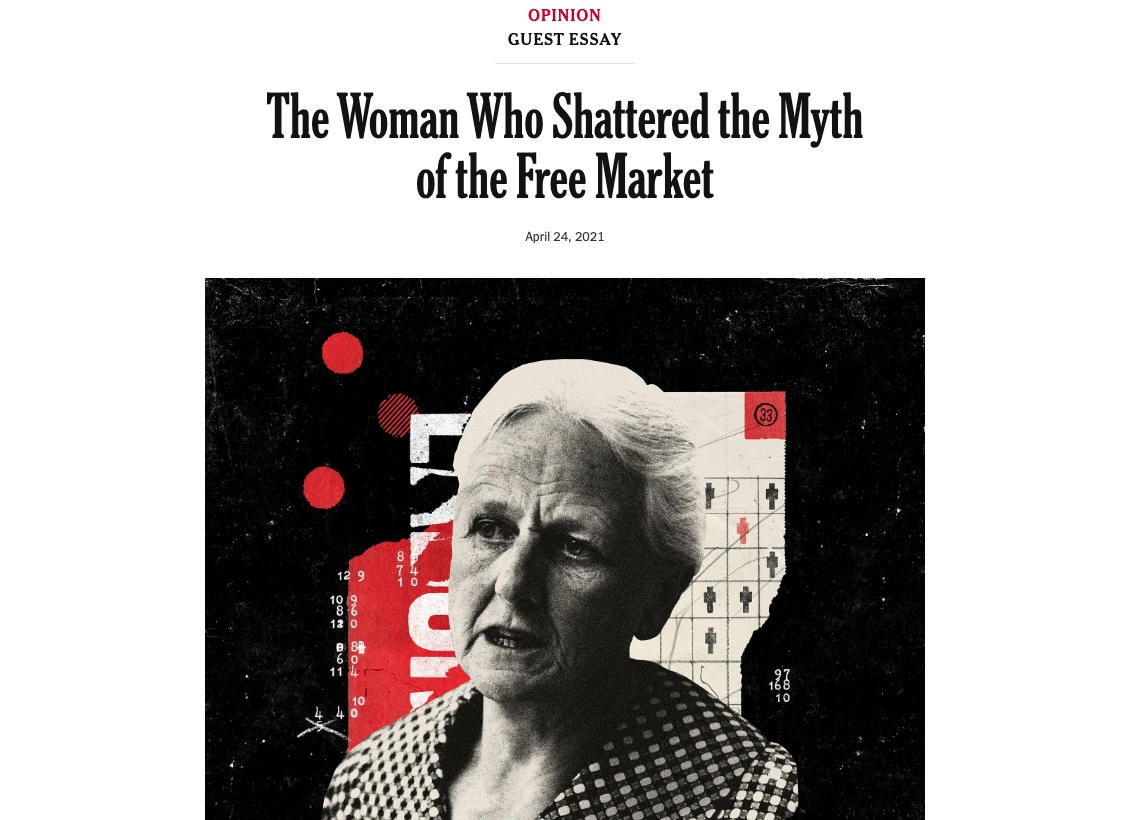
\includegraphics[width=0.6\textwidth]{aux/joan_NYT}
\end{figure}
\end{frame}
\begin{frame}
\frametitle{An important Person!}
\begin{figure}[htb]
\centering
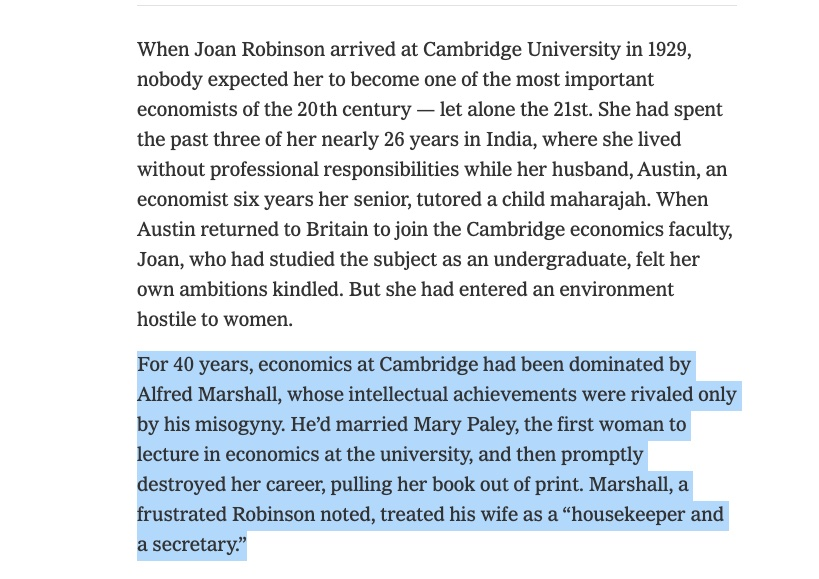
\includegraphics[width=0.6\textwidth]{aux/joan_NYT2}
\end{figure}
\end{frame}
%%
\begin{frame}
\frametitle{Taking a broader view}
\begin{itemize}
\item Monopsony useful way to model imperfect competition in labor markets.
\pause
\bigskip
\item But what does it mean to have an imperfect labor market?
\pause 
\bigskip
\item Imperfect labor market $\rightarrow$ Both employer and/or worker enjoy ``rents" from an employment relationship.
\bigskip
\begin{itemize}
\item Employer: worst off if a worker leaves, hard to replace him/her, $w<MPL$.
\bigskip
\item Employee: lost of the current job makes the worker worst off $\rightarrow$ no equal job can be found at zero cost. 
\end{itemize}
\bigskip
\item If labor markets are perfectly competitive $\rightarrow$ employers can substitute equally productive workers at the market wage. 
\begin{itemize}
\bigskip
\item And a worker who looses her job immediately finds an equal one in the labor market. 
\end{itemize}
\end{itemize}
\end{frame}
%%
\begin{frame}
\frametitle{What generates ``Rents" in a Job?}
\begin{enumerate}
\item Job differentiation.
\medskip
\item Search models.
\medskip
\begin{itemize}
\item Takes time to be matched (imperfect information about labor markets).
\medskip
\item What is exactly that workers/employers do not know? 
\medskip
\item Is this still true with Linkedin, Burning glass, etc?
\medskip
\end{itemize}
\item Institutions.
\medskip
\begin{itemize}
\item Unions.
\item Minimum Wage.
\item Collective Bargaining.
\medskip
\item Employer collusion.
\end{itemize}
\end{enumerate}
\end{frame}
%%
\begin{frame}
\frametitle{Non-Competes}
\begin{figure}[htb]
\centering
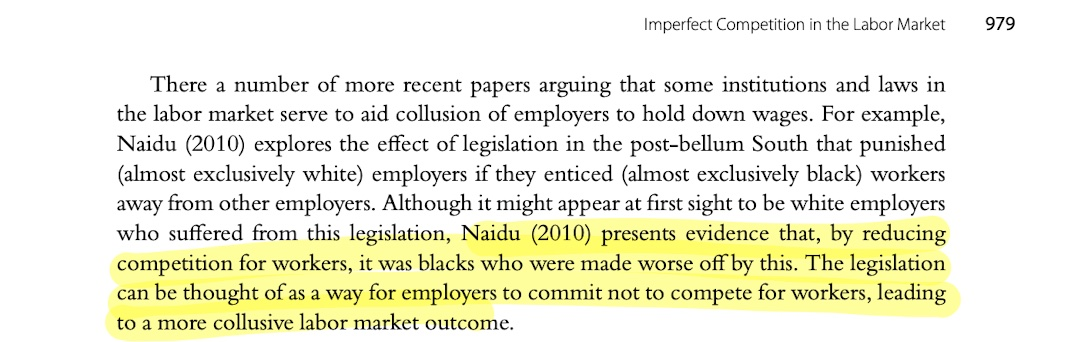
\includegraphics[width=0.7\textwidth]{aux/naidu_2010}
\end{figure}
Taken from Manning (2011) handbook chapter. 
\end{frame}
\begin{frame}
\frametitle{Non-Competes}
\begin{figure}[htb]
\centering
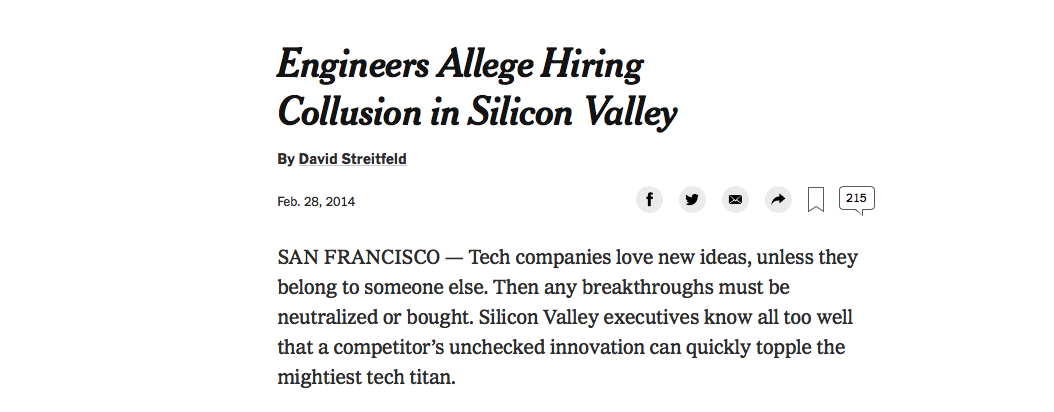
\includegraphics[width=1\textwidth]{aux/mon2}
\end{figure}
\end{frame}
%%
\begin{frame}
\frametitle{Non-Competes}
\begin{figure}[htb]
\centering
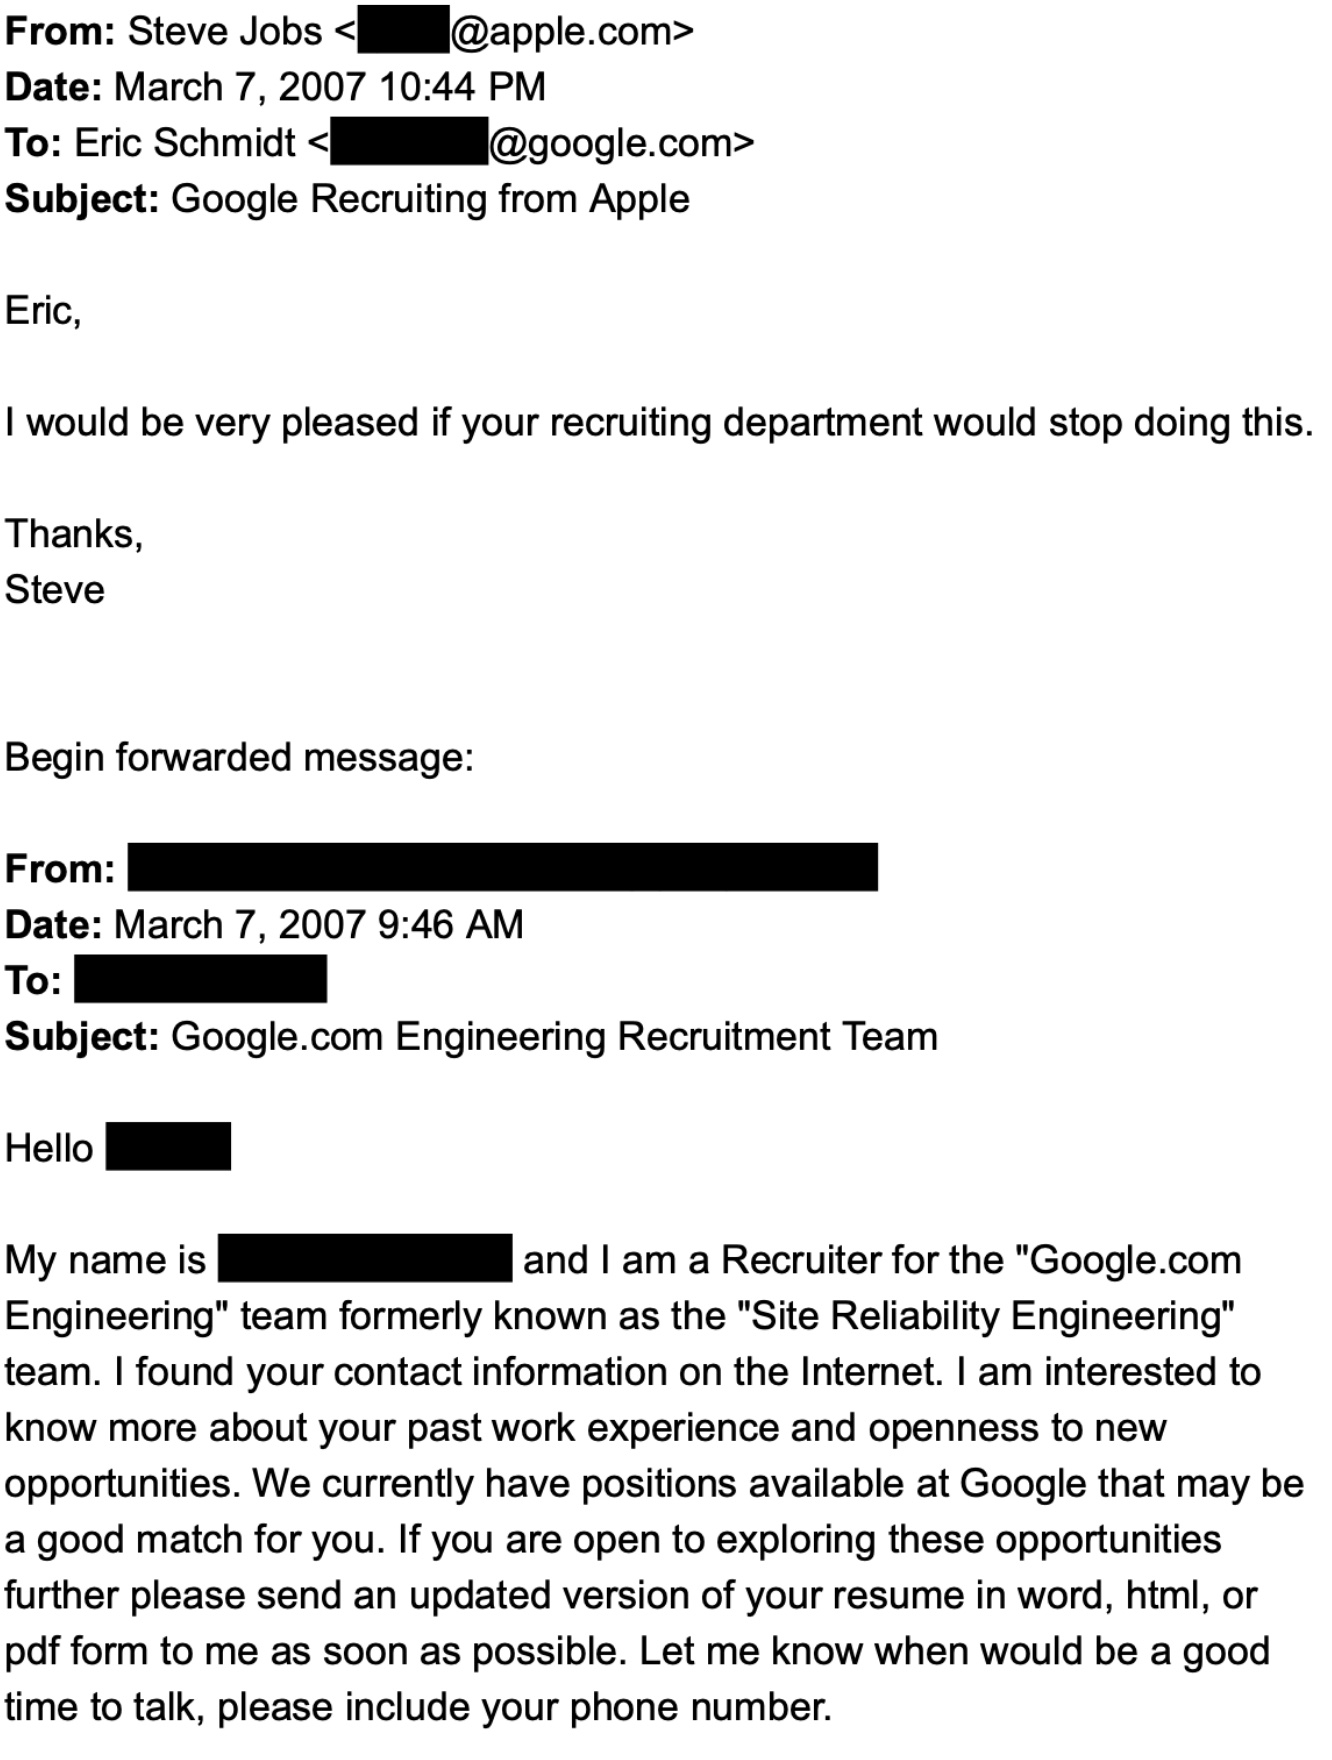
\includegraphics[width=0.5\textwidth]{aux/sj1}
\end{figure}
\end{frame}
%%
\begin{frame}
\frametitle{Non-Competes}
\begin{figure}[htb]
\centering
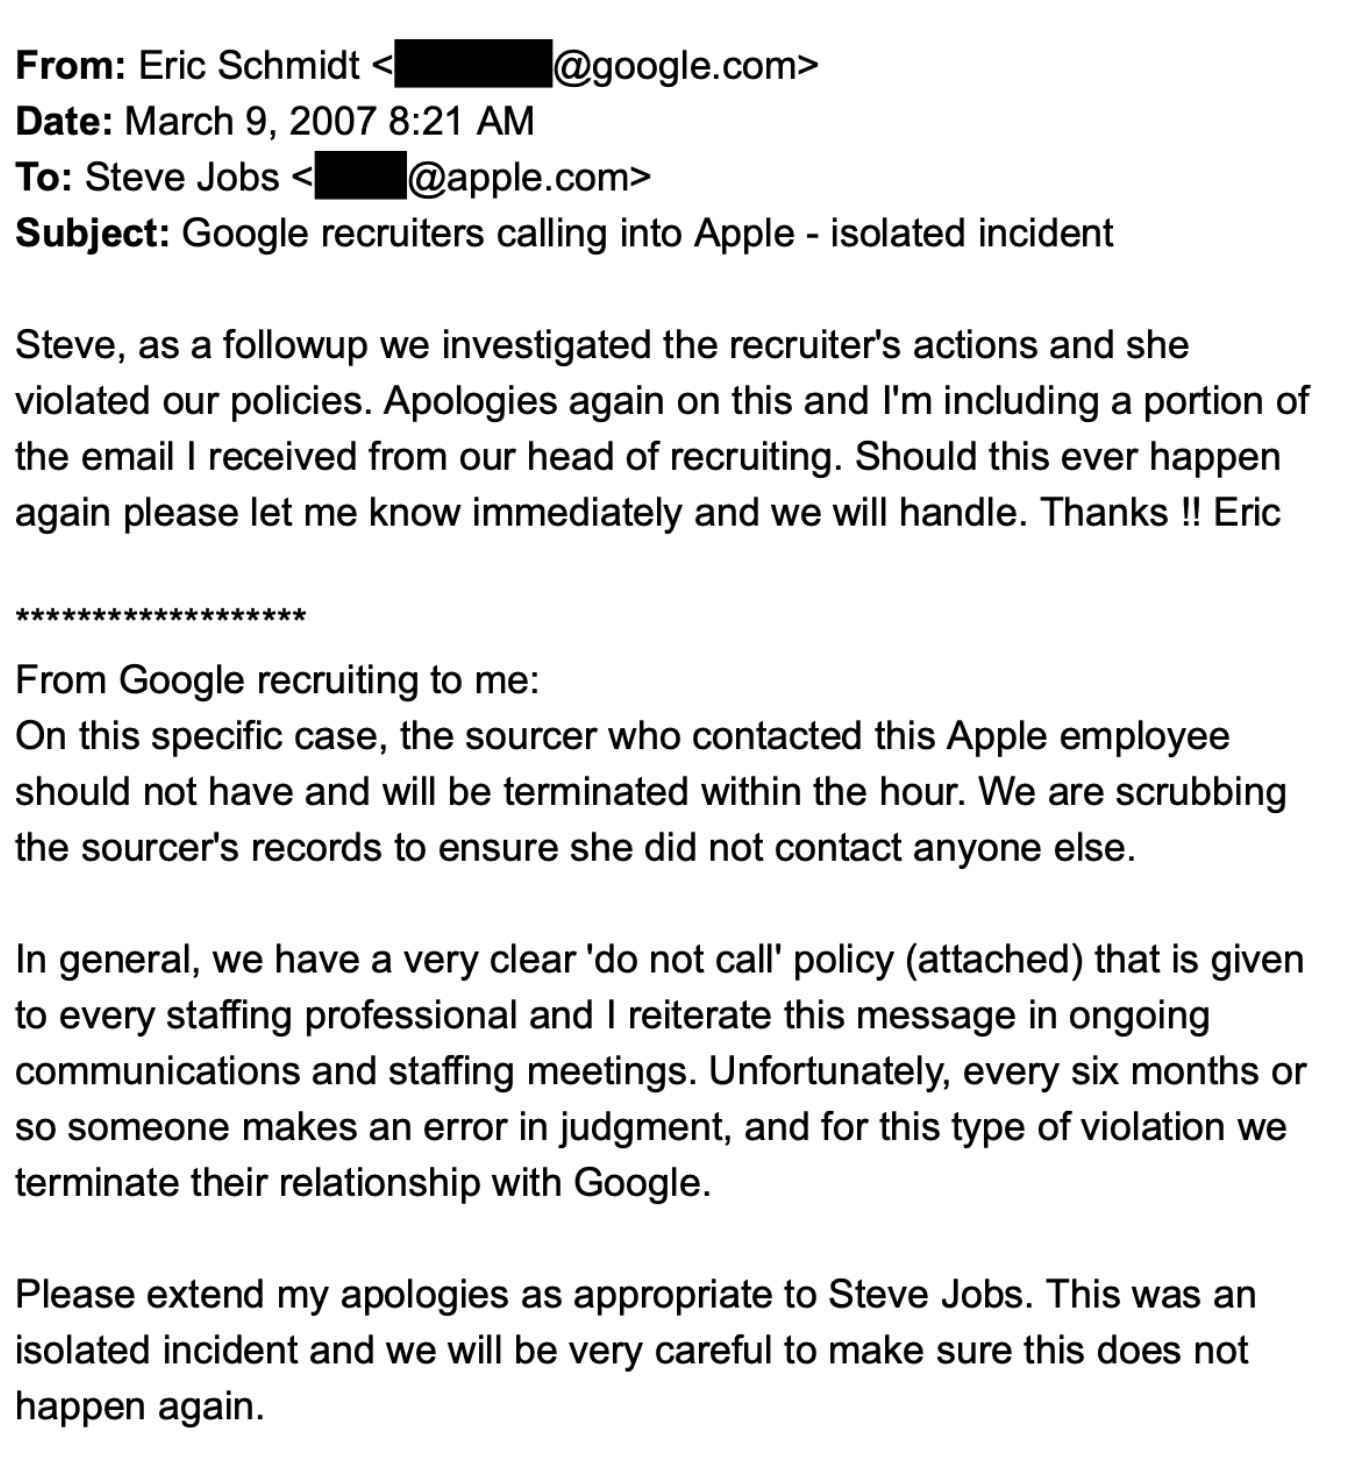
\includegraphics[width=0.5\textwidth]{aux/sj2}
\end{figure}
\end{frame}
%%
\begin{frame}
\frametitle{From Krueger and Posner, NYT Feb 2018}
\begin{figure}[htb]
\centering
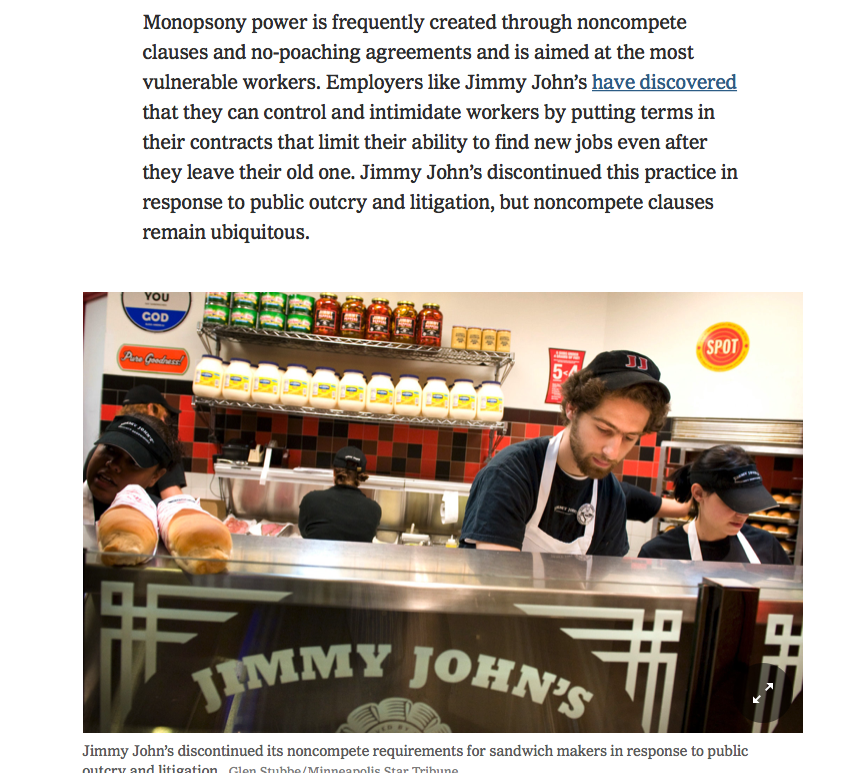
\includegraphics[width=.9\textwidth,height=0.78\textheight,keepaspectratio]{aux/mon1}
\end{figure}
\end{frame}
%%
%%
\begin{frame}
\frametitle{The legacy of Alan Krueger...}
\begin{columns}[T]
\begin{column}{0.46\textwidth}
\centering

\includegraphics[width=\columnwidth,height=0.70\textheight,keepaspectratio]{aux/mon3}
\end{column}
\begin{column}{0.52\textwidth}
\scriptsize
\textit{Interference With Employment Relations of Others.} ``During the term of this Franchise, Franchisee shall not employ or seek to employ any person who is at the time employed by McDonald's, any of its subsidiaries, or by any person who is at the time operating a McDonald's restaurant or otherwise induce, directly or indirectly, such person to leave such employment. This paragraph 14 shall not be violated if such person has left the employ of any of the foregoing parties for a period in excess of six (6) months.''
\par\medskip
\tiny
\textcolor{gray}{Source: McDonald's standard franchise agreement, Paragraph 14, as reproduced in Krueger and Ashenfelter (2022), ``Theory and Evidence on Employer Collusion in the Franchise Sector,'' \textit{Journal of Human Resources} 57(S): S324--S348.}
\end{column}
\end{columns}
\end{frame}
%%
\begin{frame}
\frametitle{Noncompetes: evidence from a field experiment}
\begin{figure}[htb]
\centering
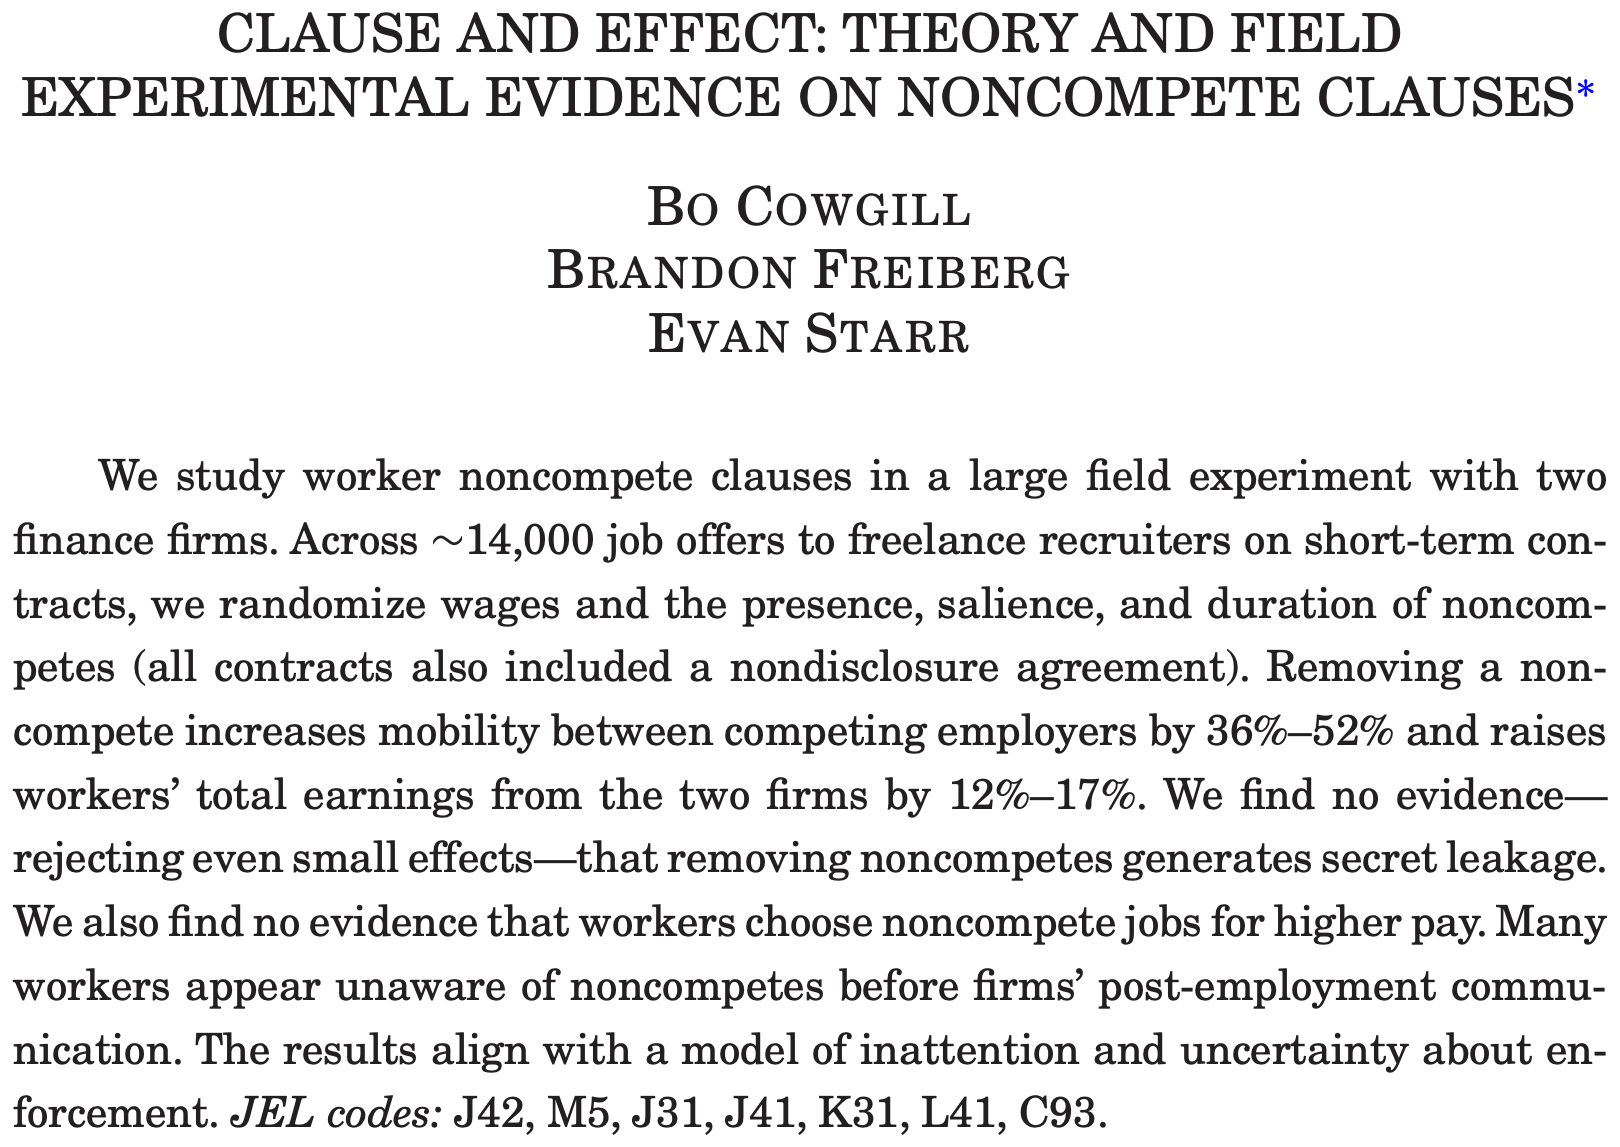
\includegraphics[width=\textwidth,height=0.78\textheight,keepaspectratio]{aux/cowgill_starr}
\end{figure}
\end{frame}
%%
\begin{frame}
\frametitle{What the paper does}
\begin{figure}[htb]
\centering
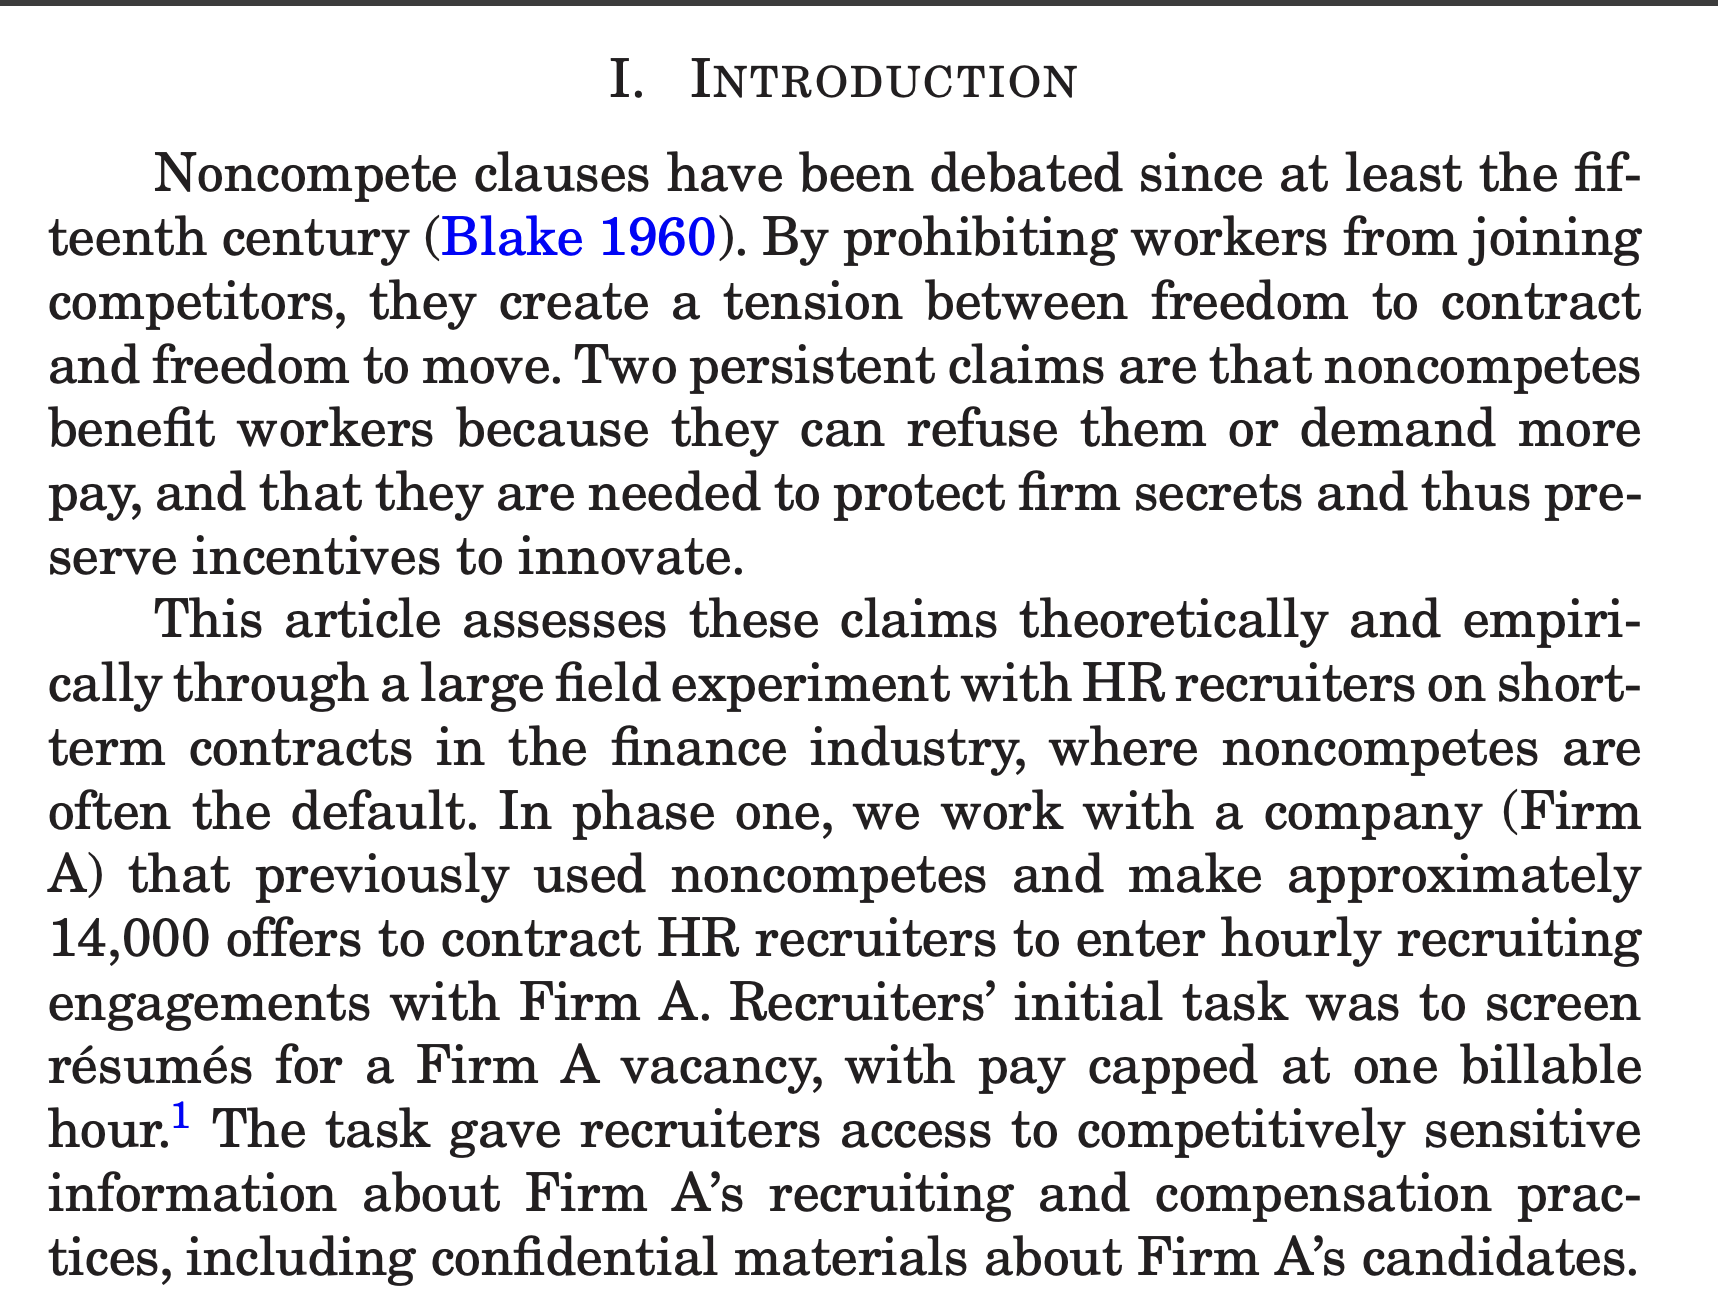
\includegraphics[width=\textwidth,height=0.80\textheight,keepaspectratio]{aux/cfs_intro1}
\end{figure}
\end{frame}
%%
\begin{frame}
\frametitle{The design}
\begin{figure}[htb]
\centering
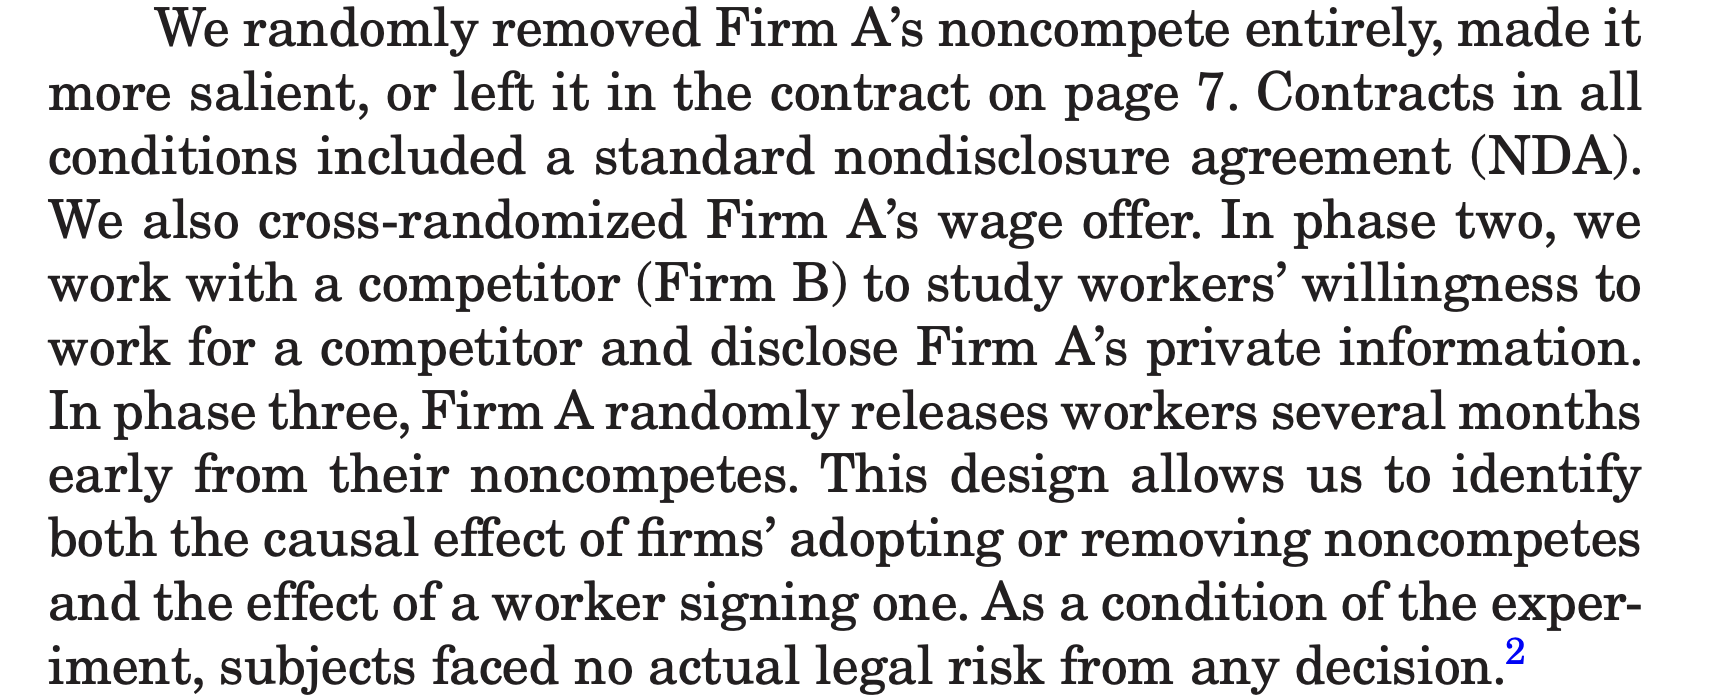
\includegraphics[width=\textwidth,height=0.72\textheight,keepaspectratio]{aux/cfs_intro2}
\end{figure}
\vfill
\tiny
\textcolor{gray}{Source: Cowgill, Freiberg and Starr, ``Clause and Effect: Theory and Field Experimental Evidence on Noncompete Clauses,'' \textit{Quarterly Journal of Economics}, Introduction.}
\end{frame}
%%
\begin{frame}{Taking Stock}
\begin{itemize}
    \item Punch line: if there are ``rents" in a job $\rightarrow$ labor markets are imperfect.
    \medskip
    \item Ideal experiment to measure the presence of ``rents"?
\end{itemize}    
\end{frame}
\begin{frame}
\frametitle{How is the pie divided?}
\begin{itemize}
\item Let's take for granted that labor markets are imperfect, i.e. there are rents in a given job. 
\medskip
\item The next question is understanding how those rents are split b/w workers and employers. 
\medskip
\item Where can we see that?
\pause
\bigskip
\item Two (but there are other) models of wage determination:
\bigskip
\begin{enumerate}
\item Ex-post wage bargaining $\rightarrow$ the wage is split after a match is realized.
\medskip
\item Ex-ante wage posting $\rightarrow$ the wage is set unilaterally by the employer before the match is realized.
\end{enumerate} 
\end{itemize}
\end{frame}
%%
\begin{frame}
\frametitle{Bargaining Model}
\begin{itemize}
\item Static approach. Assume there are firms that differ in their marginal productivity of labor, $p$. Firms can only hire one worker (from unemployment).
\bigskip
\item Worker has a leisure value equal to $b$. A firm of type $p$ chooses the wage, $w$, to maximize an asymmetric Nash bargaining criterion
\be
(p-w)^{1-\alpha}(w-b)^{\alpha}
\ee
which leads to a wage equation
\be
w=\alpha p + (1-\alpha)b
\ee
where $\alpha$ is the bargaining power of the worker (exogenous).
\bigskip
\item Ex-post efficiency (why?) but not ex-ante efficiency (hold-up problems, Grout, 1984; Acemoglu, 2001).
\end{itemize}
\end{frame}
%%
\begin{frame}
\frametitle{Posting Model}
\begin{itemize}
\item Wages are set before employers meet potential employees.
\medskip
\item For the moment assume that this meeting occurs randomly.
\medskip
\item Workers differ in their value of leisure $b$ with distribution function $\tilde{G}(.)$.
\medskip
\item Expected profit for firms 
\be
\pi(w) = (p-w)G(w).
\ee
where $G(w)=1-\tilde{G}(w)$
\item FOC for wages leads to 
\be
w(p) =\dfrac{\varepsilon(w(p))}{1+\varepsilon(w(p))}p
\ee
where $\varepsilon$ is the elasticity of the function $G()$ at the (endogenous) point $w(p)$. 
\end{itemize}
\end{frame}
%%
\begin{frame}
\frametitle{Discussion of posting models}
\begin{itemize}
\item Are all positive surplus matches realized here?
\medskip
\item Can employers perfectly price discriminate? 
\medskip
\item How should we think of $G(w)$?
\pause
\item Suppose that
\be
L(w)=G(w) = (w-b_{0})^{\varepsilon}
\ee 
which implies that
\be
w=\dfrac{\varepsilon}{1+\varepsilon}p+\dfrac{1}{1+\varepsilon}b_{0}
\ee
\pause
$\rightarrow$ elasticity of the labor supply curve to the firm $\approx$ bargaining power of workers
\end{itemize}
\end{frame}
%%
%%
\begin{frame}
\frametitle{Discussion}
\begin{itemize}
\item Which model is ``right"?
\medskip
\item Very hard question to answer empirically! No bargaining for an observed wage:
  \medskip
 \begin{itemize} 
 \item Is it because it's a posting world or the worker was prevented from bargaining? 
 \end{itemize}
  \medskip
  \pause
  \item Can you think of a moment in the data that can be used to discriminate between the two theories?
\end{itemize}
\end{frame}
%%
\begin{frame}
\frametitle{The Legacy of Alan Krueger strikes again}
\begin{figure}[htb]
\centering
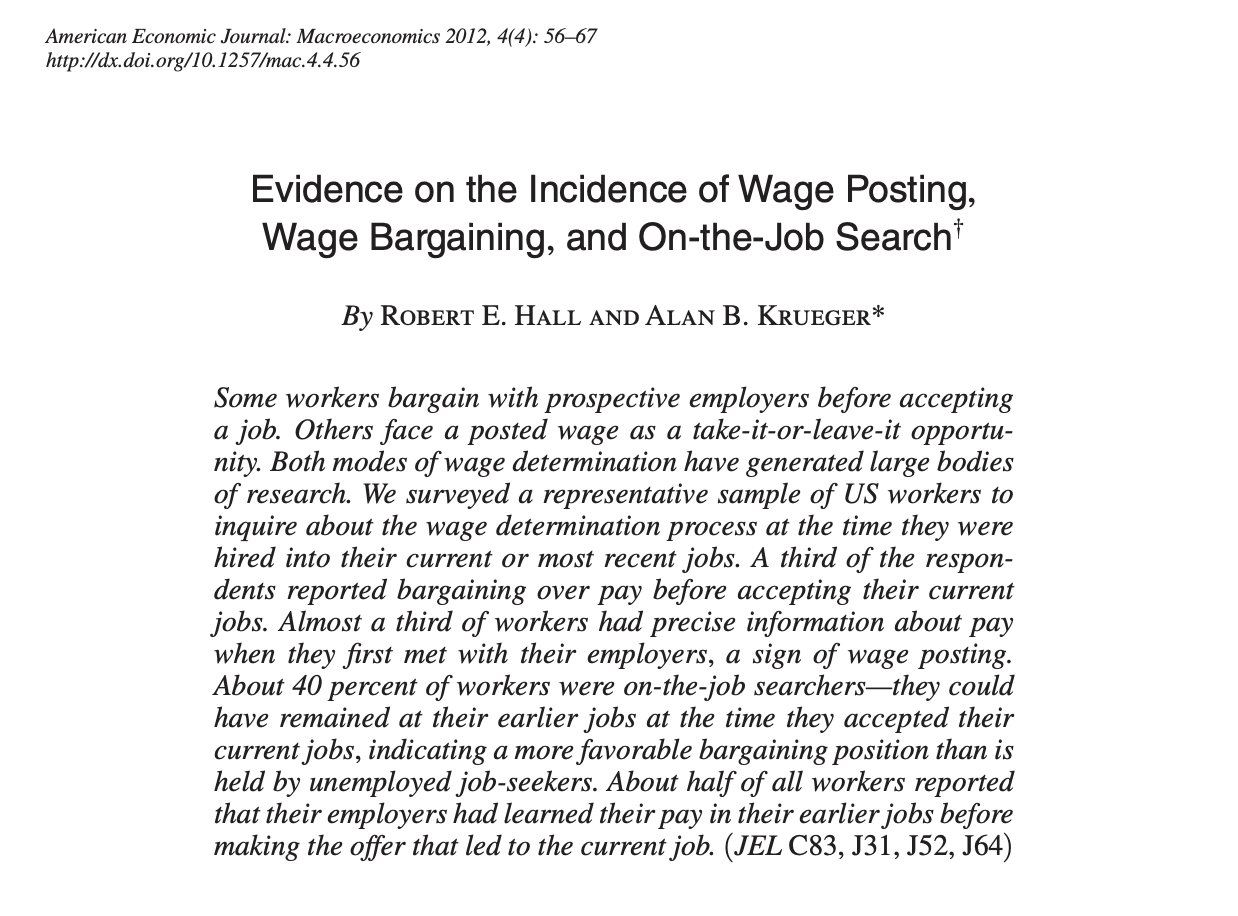
\includegraphics[width=1\textwidth,height=0.78\textheight,keepaspectratio]{aux/hall_krueger}
\end{figure}
\end{frame}
%%
\begin{frame}
\begin{figure}[htb]
\centering
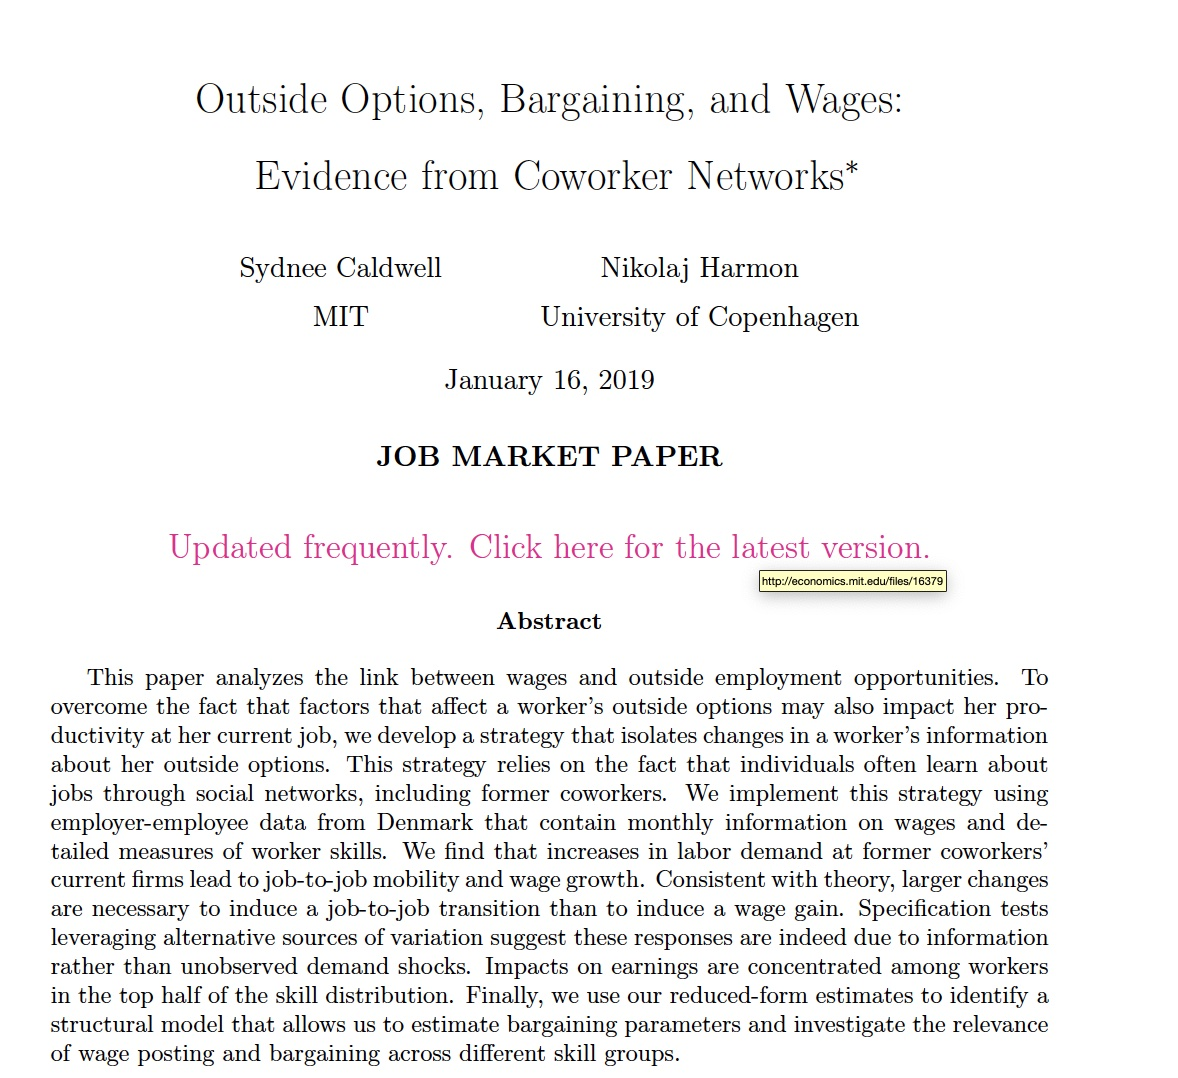
\includegraphics[width=0.7\textwidth]{aux/syde}
\end{figure}
\end{frame}
%%
\begin{frame}
\begin{figure}[htb]
\centering
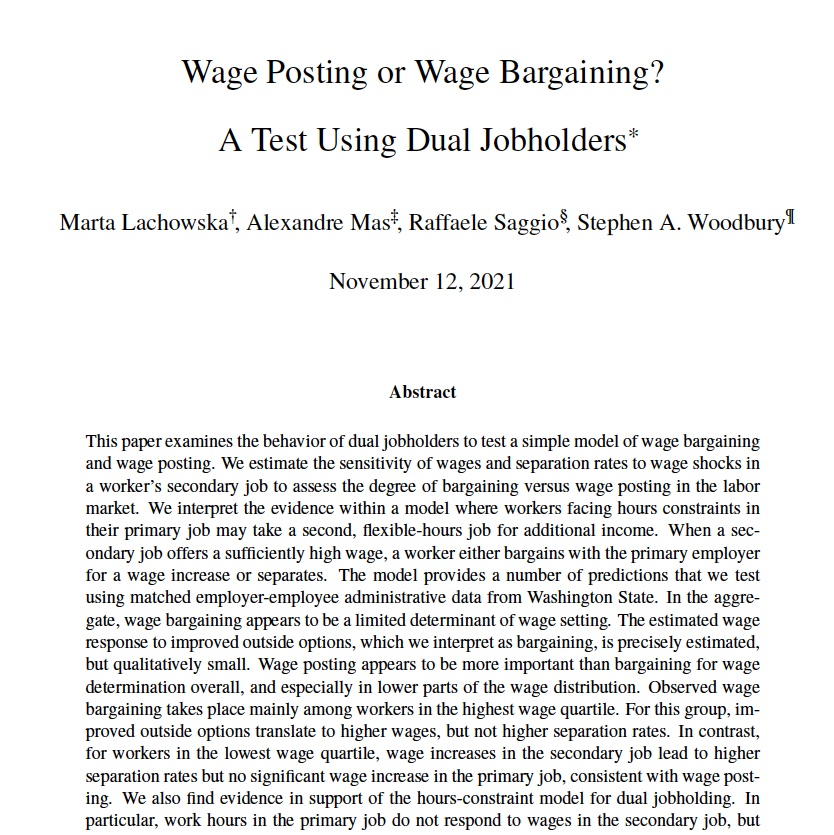
\includegraphics[width=0.7\textwidth]{aux/raffa_mas}
\end{figure}
\end{frame}
%%
%%
\begin{frame}
\begin{figure}[htb]
\centering
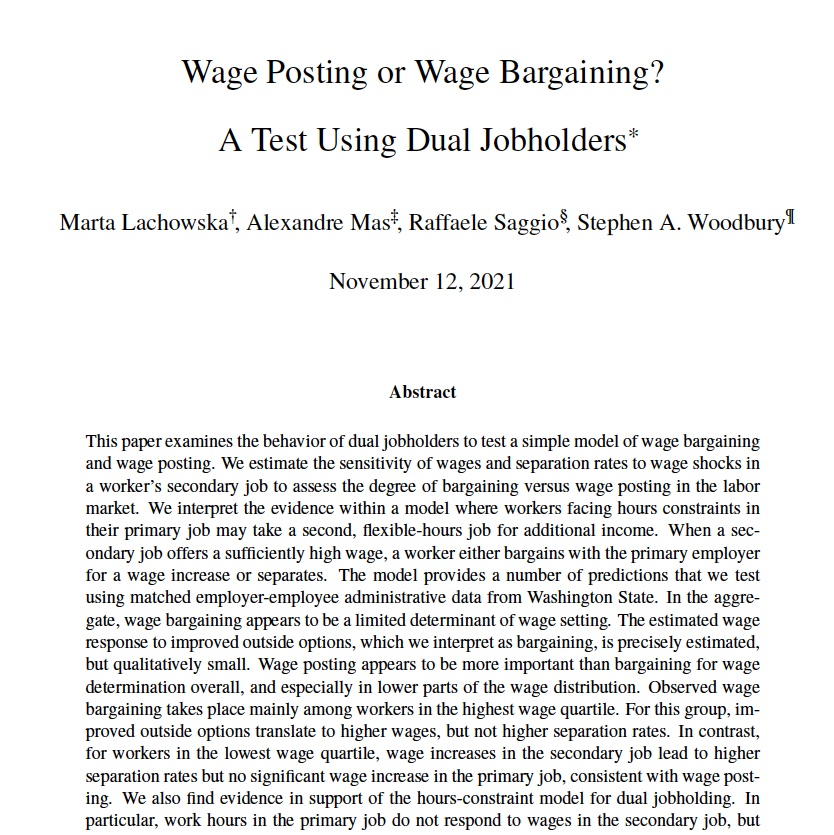
\includegraphics[width=0.7\textwidth]{aux/raffa_mas}
\end{figure}
\end{frame}
%%
\begin{frame}
\begin{figure}[htb]
\centering
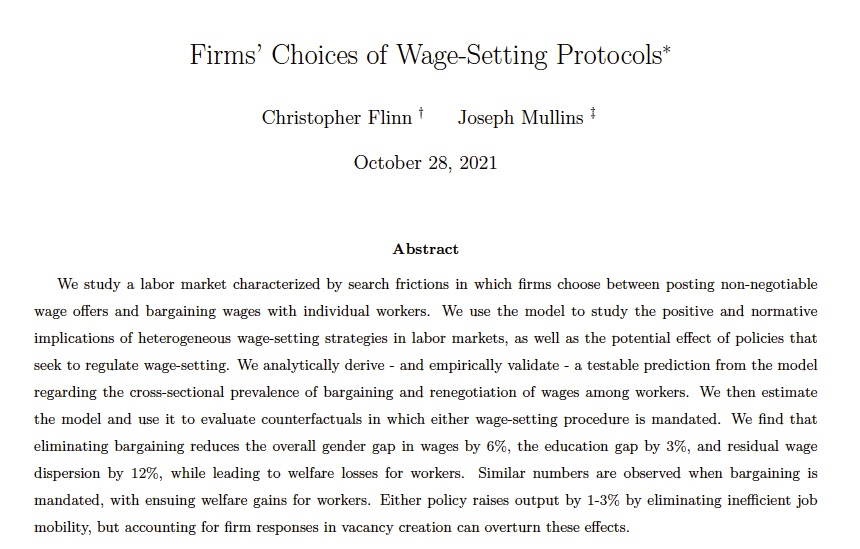
\includegraphics[width=0.7\textwidth]{aux/flinn}
\end{figure}
\end{frame}
%%
\begin{frame}
\frametitle{No model to rule them all}
\begin{figure}[htb]
\centering

\includegraphics[width=1\textwidth]{aux/lor}
\end{figure}
\end{frame}
%%%%

%%%%
\begin{frame}
\frametitle{Estimates of rent sharing}
\begin{itemize}
\item Abowd and Lemieux (1993) extension of a basic bargaining model.
\medskip
\item $F(N)$ is a revenue function that depends on the number of workers, $N$.
\medskip
\item Firms bargain with unions which have preferences $N(w-b)$ over both wages and employment
\medskip
\item Wages and employment are chosen to maximize
\be
[F(N)-wN]^{1-\alpha}[N(w-b)]^{\alpha}
\ee
which leads to
\be
F'(N) = b
\ee
\be
w= \alpha \dfrac{F(N)}{N} +(1-\alpha)b
\ee
\end{itemize}
\end{frame}
%%%%
\begin{frame}
\frametitle{Identification}
\begin{itemize}
\item Rewriting previous equation
\be
w= \alpha \dfrac{F(N)}{N} +(1-\alpha)b
\ee
\pause
\item Would OLS work here?
\medskip
\item Which IV would you use here?
\medskip
\item Which sample would you use here?
\end{itemize}
\end{frame}
%%
\begin{frame}
\frametitle{Some estimates}
\begin{figure}[htb]
\centering
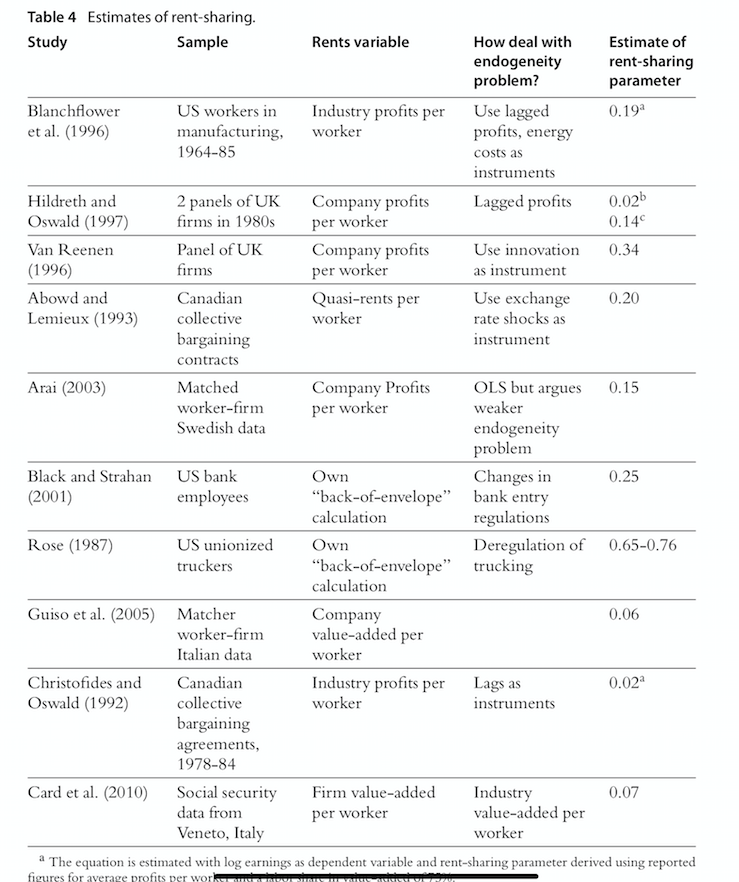
\includegraphics[width=0.6\textwidth,height=0.78\textheight,keepaspectratio]{aux/review}
\end{figure}
\end{frame}
%%

%%%% ---- begin CCHK block, brought over from Firms.tex ----
\begin{frame}
\label{cchk}
\frametitle{Card, Cardoso, Heining and Kline (2018)}
\begin{itemize}
\item Wages are set by employers to maximize profits, subject to labour supply constraints. 
\medskip
\item No search frictions, No ``unemployment".
 \medskip
 \item Workers value employers differently. This gives firms ``market power".
  \medskip
  \item CCHK model provides an important theoretical framework to link together rent sharing, monopsony models and firm inequality literature (next topic). 
\end{itemize}
\end{frame}
%%
\begin{frame}
\frametitle{Setup}
\begin{itemize}
\item $J$ firms and two types of workers: $L$ and $H$. 
\medskip
\item Each firm \underline{posts} a pair of wages $(w_{L_{j}},w_{H_{j}})$
 \medskip
 \item Workers observe the wages (costlessly). 
  \medskip
  \item Firms provide different ``workplace" environments over which workers have heterogenous preferences
  \be
  u_{i,S,j} = \beta_{S}\log(w_{S_{j}}-b_{S})+a_{S_{j}} + \epsilon_{i,S,j}
  \ee
  \item   $u_{i,S,j}$ indirect utility of worker $i$ in skill group $S$ if she works for firm $j$.
    \item   $w_{S_{j}}$ wage offered by firm $j$ to individuals in group $S$.
        \item   $b_{S}$ outside offer (e.g. wage paid in competitive industry).
         \item   $\epsilon_{i,S,j}$ idiosyncratic preferences (Type-I distributed). 
\end{itemize}
\end{frame}
%%
\begin{frame}[shrink=20]
\frametitle{Setup}
\begin{itemize}
\item Probability that a worker of type $S$ will show up at firm $j$ if this firm sets wage $w_{S_{j}}$?
\be
p_{S_{j}} \equiv \Pr\left(\argmax_{k\in\{0,\hdots,J\}}u_{iSk}=j\right) =\dfrac{\exp(\beta_{S}\log(w_{S_{j}}-b_{S})+a_{S_{j}})}{\sum_{k=1}^{J}\exp(\beta_{S}\log(w_{S_{k}}-b_{S})+a_{S_{k}})}
\ee
\item Trick: If $J$ is large then logit probabilities are well approximate by exponential probabilities
\be
p_{S_{j}} = \lambda_{S}\exp(\beta_{S}\log(w_{S_{j}}-b_{S})+a_{S_{j}})
\ee
where $\lambda_{S}$ constant common across all firms.
\medskip
\item If there is a total of $\mathcal{L}$ of low-skilled workers, then the labor supply of low-skilled workers that firm $j$ faces is given by
\be
\log(L_{j}(w_{L_{j}}))=\log(\lambda_{L}\mathcal{L}) + \beta_{L}\log(w_{L_{j}}-b_{L}) + a_{L_{j}}
\ee
Similarly for high-skilled workers
\be
\log(H_{j}(w_{H_{j}}))=\log(\lambda_{L}\mathcal{H}) + \beta_{H}\log(w_{H_{j}}-b_{H}) + a_{H_{j}}
\ee
\end{itemize}
\end{frame}
%%%%
%%
\begin{frame}
\frametitle{Firm Optimization}
\begin{itemize}
\item Firms cannot observe workers' preferences but have knowledge of their supply function.
\medskip
\item Assume that firms are price takers in the product market for the moment
\medskip
\item Output is produced according to
\be
Y_{j} = T_{j}f(L_{j},H_{j})
\ee
\medskip
\item where f(.,.) has CRS and we let $f_{S}\equiv\dfrac{\partial f(L_{j},H_{j})}{\partial S}$ for $S\in\{H,L\}$
\medskip
\pause
\item Firm problem
\be
\min_{w_{L_{j}},w_{H_{j}}} w_{L_{j}}L_{j}(w_{L_{j}}) + w_{H_{j}}H_{j}(w_{H_{j}}) \qquad s.t. T_{j}f(L_{j}(w_{L_{j}}),H_{j}(w_{H_{j}})) \geq \bar{Y}
\ee
\end{itemize}
\end{frame}
%%%%
\begin{frame}
\frametitle{Back to something familiar...}
\begin{itemize}
\item Taking FOC and rearranging, we obtain that
\be
w_{S_{j}} = \dfrac{1}{1+\beta_{S}}b_{S} + \dfrac{\beta_{S}}{1+\beta_{S}}T_{j}f_{S}\underbrace{\mu_{j}}_{\text{Marginal Cost of production}}
\ee
\medskip
\item What happens as $\beta_{S}\rightarrow\infty?$
\medskip
\item Who is capturing rents here and why? 
\medskip
\item Are amenities influencing the wage? Is this a standard compensating differential story?
\end{itemize}
\end{frame}
%%%%
\begin{frame}
\frametitle{A simple benchmark: linear production function}
\begin{itemize}
\item Suppose that we have a linear production function and that a firm faces a fixed output price $P_{j}^{0}$.
\be
Y_{j} = T_{j} N_{j}=T_{j}((1-\theta)L_{j}+\theta H_{j})
\ee
\medskip
\item Expression for wage of low skilled then becomes:
\be
w_{L_{j}} = \dfrac{1}{1+\beta_{L}}b_{L} + \dfrac{\beta_{L}}{1+\beta_{L}}T_{j}P_{j}^{0}(1-\theta)
\ee
\item Further assume that $b_{L}=(1-\theta)b$ and $b_{H}=\theta b$. Then
\be
\ln w_{L_{j}} = \ln \dfrac{(1-\theta)b}{1+\beta_{L}} + \ln(1+\beta_{L}R_{j})
\ee
\be
\ln w_{H_{j}} = \ln \dfrac{\theta b}{1+\beta_{H}} + \ln(1+\beta_{H}R_{j})
\ee
where $R_{j}\equiv \dfrac{T_{j}P_{j}^{0}}{b}$
\end{itemize}
\end{frame}
%%%%
\begin{frame}
\frametitle{Discussion of the CCHK model}
\begin{enumerate}
\item No dynamics. 
\bigskip
\item No interactions $\rightarrow$ but if it is a small market a shock to a firm's productivity will affect all other firms! 
\bigskip
\item No compensating differentials! (will come back to this)
\end{enumerate}
\end{frame}
%%%%
\begin{frame}
\frametitle{What is the punch line?}
\begin{itemize}
\item Monopsonistic posting wage models $\rightarrow$ firms suddenly matters to explain wage inequality $\rightarrow$ typically neglected in SBTC and S-D-I models
\medskip
\item These ``firm effects" are going to be highly correlated with measures of firm productivity.
\medskip
\item Firm effects only arise due to the presence of ``frictions" in the labor market.  
\medskip
\item Many things can generate monopsony power of firms!
\medskip
\item Key insight: we can infer degree of market power of firms by looking at magnitude of pass-through of ``productivity" shocks into wages. 
\medskip
\item Example that do this really well:  Kline, Petkova, Williams, Zidar (2019); Garin and Silverio (2023)
\end{itemize}
\end{frame}
%%%% ---- end CCHK block ----
%%
\begin{frame}
\frametitle{Dube, Jacobs, Naidu, Suri(2018): Monopsony in online labor markets}
\begin{itemize}
\item Emergence of \textit{digital} platforms, e.g. Uber, TaskRabbit or Amazon Mechanical Turk.
\bigskip
\item Are these labor markets have a higher/lower degree of market power?
\bigskip
\pause
\item Dube et al. formally test the degree of market-power in Amazon Mechanical Turk platform. 
\end{itemize}
\end{frame}
%%
\begin{frame}
\begin{figure}[htb]
\centering
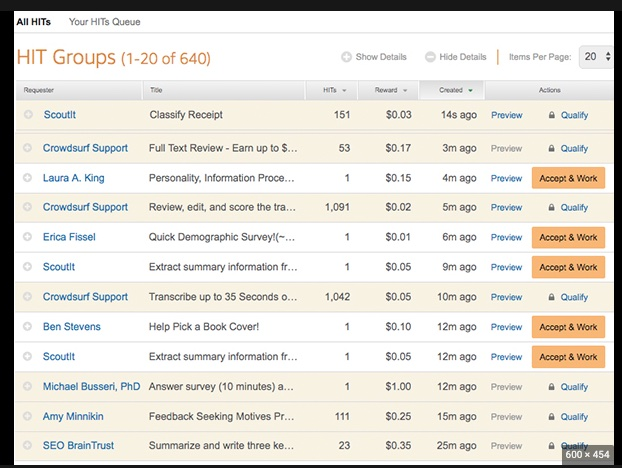
\includegraphics[width=1\textwidth]{aux/turk3}
\end{figure}
\end{frame}
\begin{frame}
\begin{figure}[htb]
\centering
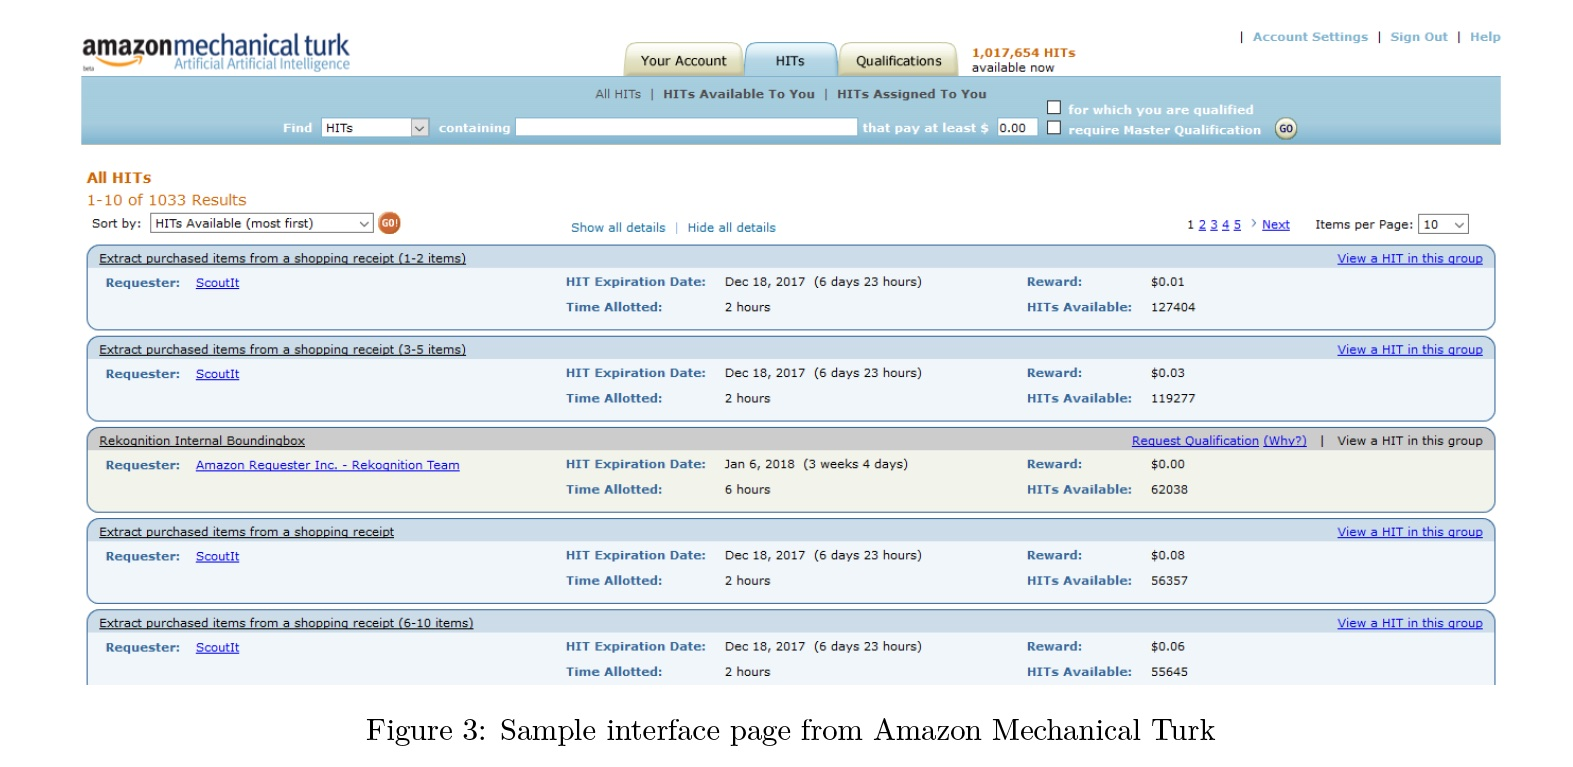
\includegraphics[width=1\textwidth]{aux/turk}
\end{figure}
\end{frame}
\begin{frame}
\frametitle{Dube, Jacobs, Naidu, Suri(2018): Monopsony in online labor markets}
\begin{itemize}
\item Scraped the universe of tasks (HIT) posted on Amazon MTurk.
\bigskip
\item Also used data from previous experiments where other people have randomized the wage associated to a given task posted on Amazon MTurk. 
\bigskip
\pause
\item Nice methodological contribution: comparison of experimental estimates with traditional regression techniques (Fixed effects regressions) as well as Machine Learning Techniques (Double Machine Learning Lasso covered in 628). 
\end{itemize}
\end{frame}
%%
\begin{frame}
\frametitle{Monopsony in a task market}
\begin{itemize}
\item Go back to our original discussion on monopsony. 
\medskip
\item Suppose an employer posts a job in MTurk that is 1 dollar (per hour) lower than all the jobs observed in the platform. 
\medskip 
\item Why do you think someone might take such a job? 
\medskip
\end{itemize}
\end{frame}
%%
%%
\begin{frame}
\frametitle{Empirical model}
\begin{itemize}
\item Scraper from 2014-2017 of MTurk platoform
\medskip
\item $duration_{h}\equiv$ how long a task remained in the platform. 
\item $reward_{h}\equiv$ observed reward for completing the task. 
\medskip
\item First empirical model (FE):
\be
\log(duration_{h}) = -\eta_{1}\log(reward_{h})+\rho_{r(h)} + \tau_{t(h)} + \delta_{d(h)} + \epsilon_{h}
\ee
$\rho_{r(h)}\equiv$ requester's FE.
$\delta_{d(h)}\equiv$ deciles of the time allotted by the requester.
  $\tau_{t(h)}\equiv$ time fixed effect
\item Double-ML:
\be
\log(duration_{h}) = -\eta_{1}\log(reward_{h})+\underbrace{g(Z_{h})}_{\E[\log(duration_{h})\vert Z]}+ \epsilon_{h}
\ee
+experimental evidence.
\end{itemize}
\end{frame}
%%
\begin{frame}{Rich set of features}
\begin{figure}[htb]
\centering
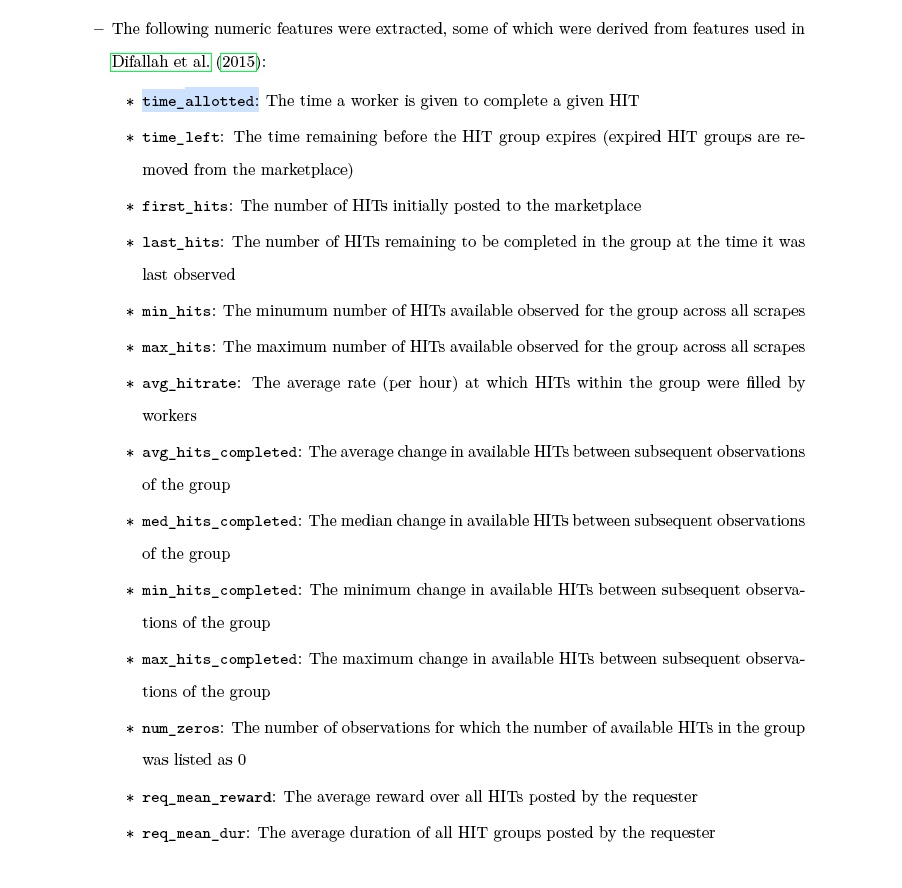
\includegraphics[width=1\textwidth,height=0.78\textheight,keepaspectratio]{aux/turk1}
\end{figure}
\end{frame}
\begin{frame}{Rich set of features}
\begin{figure}[htb]
\centering
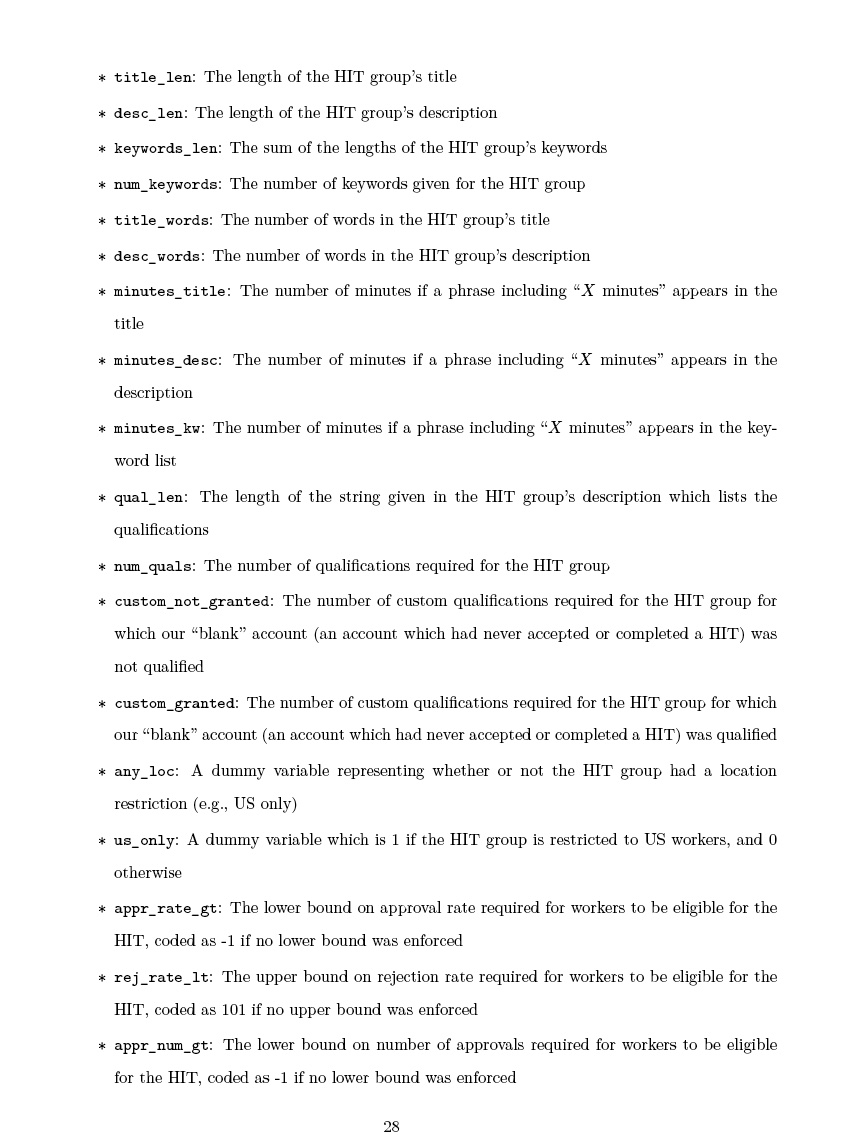
\includegraphics[width=1\textwidth,height=0.78\textheight,keepaspectratio]{aux/turk2}
\end{figure}
\end{frame}
%%
\begin{frame}
\frametitle{FWL 2.0 }
\begin{figure}[htb]
\centering
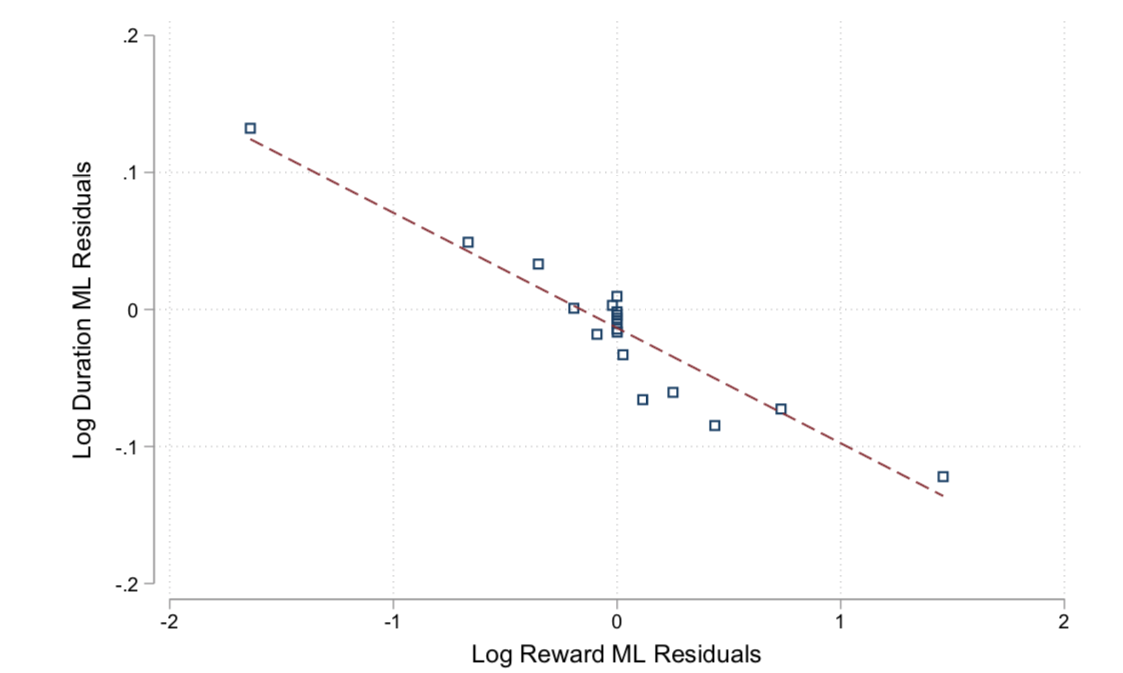
\includegraphics[width=1\textwidth]{aux/dube11}
\end{figure}
\end{frame}
%%
\begin{frame}
\frametitle{FE $\approx$ ML}
\begin{figure}[htb]
\centering
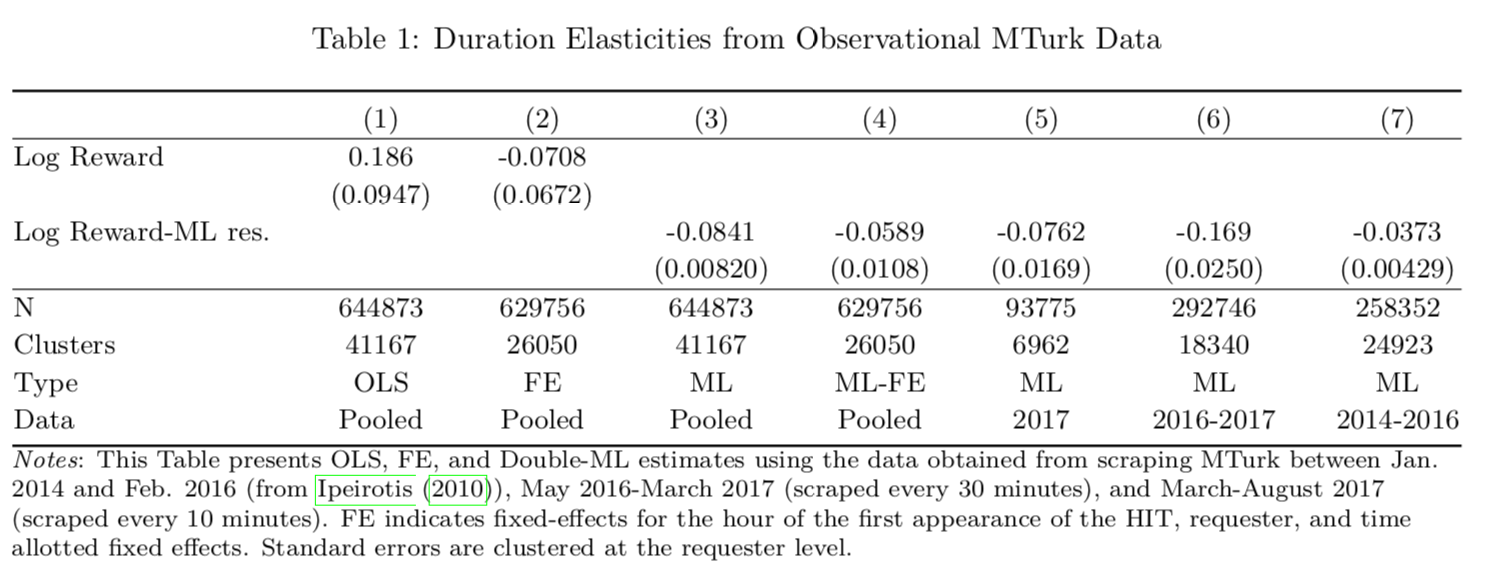
\includegraphics[width=1\textwidth,height=0.56\textheight,keepaspectratio]{aux/dube12}
\end{figure}
\vfill
\footnotesize
Not in Table 1: using the \emph{experimental} data, the precision-weighted mean labour supply elasticity facing a requester is \textcolor{red}{$0.14$}. The pooled recruitment elasticity on its own is $0.06$, against the $0.08$ of the preferred double-ML specification.
\par\smallskip
\tiny
\textcolor{gray}{Source: Dube, Jacobs, Naidu and Suri (2020), ``Monopsony in Online Labor Markets,'' \textit{American Economic Review: Insights} 2(1): 33--46. The $0.14$ is the precision-weighted mean experimental elasticity reported in Figure 2 of the NBER WP 24416 version of the paper.}
\end{frame}
%%%%
\end{document}

